\documentclass[journal]{IEEEtran}

\usepackage{pdfpages}
\usepackage{cite}

\usepackage{amsthm}
\usepackage{lipsum} % for filler text
\newtheorem{theorem}{Theorem}
\usepackage{color}
\usepackage[caption=false,font=footnotesize]{subfig}
\newcommand{\subparagraph}{}

\usepackage{amssymb,amsmath}

%\usepackage[compact]{titlesec}
%\titlespacing{\section}{5pt}{2pt}{2pt}
%\titlespacing{\subsection}{5pt}{2pt}{2pt}

%\setlength\floatsep{5pt plus 0.5pt minus 0.5pt}
%\setlength\dblfloatsep{3pt plus 0.5pt minus 0.5pt}
%\setlength\intextsep{2pt plus 0.5pt minus 0.5pt}
\setlength\textfloatsep{15pt plus 1pt minus 1pt}
%\setlength\dbltextfloatsep{5pt plus 1pt minus 1pt}
\setlength\abovecaptionskip{3pt plus 0.5pt minus 0.5pt}
%\setlength\belowcaptionskip{1pt plus 0.5pt minus 0.5pt}
%\setlength\abovedisplayskip{1pt plus 1pt minus 1pt}
%\setlength\belowdisplayskip{1pt plus 1pt minus 1pt}


\makeatletter
\def\hlinewd#1{%
\noalign{\ifnum0=`}\fi\hrule \@height #1 %
\futurelet\reserved@a\@xhline}
\makeatother
\usepackage[binary-units=true]{siunitx}
\usepackage[algoruled,noline,longend,linesnumbered]{algorithm2e}

\usepackage{graphicx}
\usepackage{pgfplots}

\thinmuskip=2mu 
\medmuskip=2mu plus 2mu minus 2mu
\thickmuskip=2mu plus 1mu minus 1mu

\begin{document}


\graphicspath{{Fig/}}
\def\figname{Fig.}
\def\algname{Algorithm}
\newcommand{\figurefontsize}{\footnotesize}
\newcommand{\papertitle}{Test Generation for Flow-Based Microfluidic
Biochips with General Architectures}
\newcommand{\tum}{Technical University of Munich (TUM)}

\setcounter{page}{0} 
\pagenumbering{roman}



\clearpage
\thispagestyle{empty} 
\begin{table*}
\begin{center}
\begin{minipage}[t][21.5cm][t]{12.8cm}
%\fontsize{10}{10}\selectfont
\renewcommand{\baselinestretch}{1.2} 
\normalsize


\vspace{10pt}

Dear Editors, dear Reviewers,\\

\vspace{3pt}

Enclosed please find our manuscript entitled \textit{\papertitle}. We submit this
manuscript as a regular paper for publication in \textit{IEEE Transactions on
Computer-Aided Design of Integrated Circuits and Systems}.
%for publication in the Special Issue on Deep Physical Design Techniques for
%Next Generation Technologies, IEEE Transactions on Computer-Aided Design of
%Integrated Circuits and Systems.

\vspace{3pt}

This work builds on the method in the appended paper, which was published at the 
\textit{Design, Automation and Test in Europe} Conference in 2017 as [1].
In this manuscript, we enhance the previous work as follows: 

\vspace{3pt}

\begin{enumerate} 

  \item The model for testing Fully Programmable Valve Arrays (FPVAs) in [1] 
    has been extended to take advantage of multiple test
    ports to improve test efficiency. Accordingly, the number of test patterns
    can be decreased by up to 50\%, leading to a significant
    reduction of test cost. This extension is described in
    Section~\ref{sec:multiple_port_tree} and Section~\ref{sec:multiple_port_cut}.

  \item The extended test model is capable of generating test patterns for
    traditional flow-based microfluidic biochips, and the number of the
    resulting test patterns is much smaller than that from the other previous
    method based on ATPG, as described in Section~\ref{sec:adapt_traditional}.
   
  \item In the extension, test of control layer leakage is covered with additional
    constraints and explained in detail in Section~\ref{sec:control_layer_test}.
    In addition, long channels and obstacles are merged to facilitate 
    the generation of test patterns, as described in detail in Section~\ref{sec:walls_holes}. 

  \item Furthermore, a loop relaxation technique is introduced to improve the scalability of the
    original model based of ILP. Constraint violations are addressed by
    amending the test patterns to improve the efficiency of test
    generation. Consequently, large designs can be dealt with using this
    enhanced method, as described in Section~\ref{sec:loop_relax}.

  \item Simulation results have been extended according to the new improvements 
    to demonstrate their effectiveness and efficiency.

\end{enumerate} 

%\vspace{-10pt}
%We confirm that this manuscript has not been published or submitted elsewhere
%and all authors have approved the manuscript and agree with the submission.\\

\vspace{10pt}


We look forward to hearing from you 
and thank you very much for your time and consideration.


\vspace{25pt}

Yours sincerely,

\vspace{10pt}
Chunfeng Liu, Bing Li, Bhargab B. Bhattacharya, Krishnendu Chakrabarty,
Tsung-Yi Ho and Ulf Schlichtmann \\



\end{minipage}
\end{center}
\end{table*}

\clearpage
%\thispagestyle{empty} 
%\mbox{}
%\clearpage
\setcounter{page}{0} 
\pagenumbering{arabic}



\title{\papertitle}

\author{	
Chunfeng Liu, Bing Li, Bhargab B. Bhattacharya, Krishnendu
Chakrabarty, Tsung-Yi Ho, and Ulf Schlichtmann

\thanks{A preliminary version of this paper was published as \cite{CBBK17} in
the Proceedings of the Design, Automation and Test in Europe (DATE)
conference, 2017. The improvements include an acceleration technique with loop
relaxation, test of leakage in the control layer and test of chips with multiple
pressure sensors.}
          \thanks{Chunfeng Liu, Bing Li and Ulf Schlichtmann are with the Chair
	    of Electronic Design Automation,
          \tum, Munich 80333, Germany (e-mail: chunfeng.liu@tum.de; b.li@tum.de;
  ulf.schlichtmann@tum.de).}
          \thanks{Bhargab B. Bhattacharya is with the Indian Statistical Institute, Kolkata, India
   (e-mail: bhargab@isical.ac.in).}
           \thanks{Krishnendu Chakrabarty is with the Department of 
	     Electrical and Computer Engineering and the Department of Computer
	     Science, Duke University, Durham, NC, USA (e-mail: krish@ee.duke.edu).}
            \thanks{Tsung-Yi Ho is with the Department of Computer Science,  
	    National Tsing Hua University, Hsinchu, Taiwan (e-mail: tyho@cs.nthu.edu.tw).}
}

\maketitle
 \markboth{IEEE TRANSACTIONS ON COMPUTER-AIDED DESIGN OF INTEGRATED CIRCUITS AND SYSTEMS}
 {Liu \MakeLowercase{\textit{et al.}}: \papertitle}

 
 \IEEEpeerreviewmaketitle

%\thispagestyle{fancy}

\begin{abstract}

Flow-based microfluidic biochips have attracted much attention in the EDA community due to their miniaturized size and execution efficiency. Previous research, however, still follows the traditional
computing model with a dedicated storage unit, which actually becomes a bottleneck of the performance of biochips. In this paper, we propose a distributed channel-storage architecture (DCSA) to cache fluid samples inside flow channels temporarily.
Since distributed storage can be accessed more efficiently than a dedicated storage unit and channels can switch between the roles of transportation and storage easily, biochips with this architecture can achieve a higher execution efficiency even with fewer resources. Furthermore, we also address the flow-path planning that enables the manipulation of actual fluid transportation/caching on a chip. Simulation results confirm that the execution efficiency of a bioassay can be improved by up to 28\%, while the number of valves in the biochip can be reduced significantly. Also, flow paths for transportation tasks can be constructed and planned automatically with minimum extra resources.

\begin{IEEEkeywords}
Microfluidic biochips, channel storage, scheduling, architectural synthesis, flow-path mapping.
\end{IEEEkeywords}

\end{abstract}


% this file is called up by thesis.tex
% content in this file will be fed into the main document

%: ----------------------- introduction file header -----------------------
\chapter{Introduction}

% the code below specifies where the figures are stored
\ifpdf
    \graphicspath{{1_introduction/figures/PNG/}{1_introduction/figures/PDF/}{1_introduction/figures/}}
\else
    \graphicspath{{1_introduction/figures/EPS/}{1_introduction/figures/}}
\fi

% ----------------------------------------------------------------------
%: ----------------------- introduction content ----------------------- 
% ----------------------------------------------------------------------



%: ----------------------- HELP: latex document organisation
% the commands below help you to subdivide and organise your thesis
%    \chapter{}       = level 1, top level
%    \section{}       = level 2
%    \subsection{}    = level 3
%    \subsubsection{} = level 4
% note that everything after the percentage sign is hidden from output



\section{The rise of the chip} % section headings are printed smaller than chapter names
% intro

The field of microfluidics has four parents: molecular analysis, biodefence, molecular biology and microelectronics. 
First came analysis. The distant origins of microfluidics lie in microanalytical methods — gas-phase chromatography (GPC), 
high-pressure liquid chromatography (HPLC) and capillary electrophoresis (CE) — which, in capillary format, revolutionized chemical analysis. These methods (combined with the power of the laser in optical detection) made it possible to simultaneously achieve high sensitivity and high resolution using very small amounts of sample. With the successes of these microanalytical methods, it seemed obvious to develop new, more compact and more versatile formats for them, and to look for other applications of microscale methods in chemistry and biochemistry. A second, different, motiva

The first key area that inspired the field of microfluidics is molecular analysis. 

A second, different, motivation for the development of microfluidic systems came with the realization — after the end of the cold war — that chemical and biological weapons posed major military and terrorist threats. To counter these threats, the Defense Advanced Research Projects Agency (DARPA) of the US Department of Defense supported a series of programmes in the 1990s aimed at developing field-deployable microfluidic systems designed to serve as detectors for chemical and biological threats. These programmes were the main stimulus for the rapid growth of academic microfluidic technology.

The third motivational force came from the field of molecular biology. The explosion of genomics in the 1980s, followed by the advent of other areas of microanalysis related to molecular biologies, such as high-throughput DNA sequencing, required analytical methods with much greater throughput, and higher sensitivity and resolution than had previously been contemplated in biology. Microfluidics offered approaches to overcome these problems. The fourth contribution was from microe


The original hope of microfluidics was that photolithography and associated technologies that had been so successful in silicon microelectronics,
[The origins and the future of microfluidic]


Microfluidic biochips are revolutionizing the traditional biochemical experiment 
flow with their high execution efficiency and 
miniaturized fluid manipulation \cite{JEMP08, EVNR03,JMSQ07}. 
Devices are built 
%from microchannels and valves 
in such a chip to execute specific operations, such as mixing and detection.
Fluid samples are transported through microchannels between devices to carry
out the protocol of a bioassay. 
All these functions are performed at the nanoliter level and
controlled by a microcontroller without human intervention. 
The efficiency and reliability of such miniaturized and automated chips 
endow them with a great potential to improve human life significantly, 
and the research to bridge them with real-world applications
%bring them from prototypes in laboratories to industry production 
is key to their success.   

\begin{figure}[htpb]
    {      
    \centering
    % \input{Fig/valve_mixer_chip.pdf_tex}
    \input{1_introduction/figures/valve_mixer_chip.pdf_tex}
    %\includegraphics{Fig/valve_mixer_chip.png}
    \caption{Components and structure of flow-based biochips. 
    (a) Valves constructed at intersections of flow/control channels \cite{JMSQ07}. 
    (b) Mixer \cite{JMSQ07}. (c) A part of a biochip
    containing a mixer surrounded by a transportation channel network 
    \cite{ESWD13}.}
    \label{fig:valve_mixer_chip}
    }
    \end{figure}

A flow-based microfluidic biochip is constructed from basic components such as
%basic components, namely, 
microchannels and microvalves, henceforth named as channels and valves for
simplicity.
Flow channels are used to transport reaction samples and reagents
between different locations. Above flow channels, control 
channels are built to 
conduct air pressure to intersections of flow channels and control channels 
to form 
valves, as illustrated in \figname~\ref{fig:valve_mixer_chip}(a),
where three valves are constructed at the intersections.
These channels are built from elastic materials, so that
air pressure in a control channel can block the movement of fluid sample
by squeezing the flow channel downwards.
Conversely, if the pressure in the control channel is
released, the fluid sample can resume its movement. 
%Functionally, valves are thus formed at intersections of
%flow channels and control channels, and the open/close states
%of valves are controlled by the air pressure fed into the 
%control channels. 
Since the channel width has been miniaturized
down to 50 um \cite{Studer04} thanks to the advance of manufacturing
technology, a huge number of channels and valves can
already be integrated
into a single biochip to perform large-scale experiments and diagnoses.

With valves as basic controlling components, complex devices 
can be constructed. For example, mixers can be built using
channels and valves to execute mixing operations, which are very
common in biochemical applications. The structure of a mixer is shown
in \figname~\ref{fig:valve_mixer_chip}(b),
where the three valves at the bottom are actuated alternately by 
applying and releasing air pressure in the control
channels 
%to form a circular flow around the device 
to mix fluid samples and reagents by peristalsis.
The execution of a mixing operation in a biochip is demonstrated
in a video \cite{mixing_store}. 
After the mixing operation is completed, the resulting fluid sample 
can be stored in a dedicated storage unit temporarily. %in the biochip.

In a biochip, devices executing specific operations, e.g., mixing and heating,
are connected by channels so that intermediate reaction results %fluid samples 
can be
transported between devices for processing. All these operations and
transportation are controlled
%by valves, whose open/close states are regulated
by a microcontroller, which 
%. To execute a biochemical assay, the microcontroller 
issues instructions in a given order to actuate valves 
to move fluid samples 
%between devices 
and execute operations.
%of valve actuation to move fluid samples
%to different devices to process them. 
%The photograph of a complete biochip is
%shown 
\figname~\ref{fig:valve_mixer_chip}(c) shows a mixer (reaction loop) surrounded
by flow channels (green), control channels (yellow and red) and valves
(yellow and red blocks).
%formed 
%at their
%At the 
%intersections.
%of flow and control channels, 
%used to direct fluid transportation. 
These channels and valves together form a network similar to the
road transportation system. If fluid channels should cross, %four
valves are built %at the crossing point 
to form a switch, as shown 
in \figname~\ref{fig:valve_mixer_chip}(c).
At any moment, only two out of the four valves should be opened to 
direct fluid transportation; 
%form a flow path; 
the other two valves must be closed to avoid fluid
contamination. Consequently, the role of the valves at the intersection
of %two 
flow channels is similar to that of the traffic lights in the road
transportation system, while the open/closed states of the valves are
controlled by a microcontroller according to the protocol of the application.
%and many valves are used to coordinate fluid
%transportation and assay execution. 
The mixer and the channel network
%The size of the chip in 
in \figname~\ref{fig:valve_mixer_chip}(c)
are implemented into a biochip of the size comparable to that of a coin 
as shown %in the photo 
at the upper left
corner, %of \figname~\ref{fig:valve_mixer_chip}(c), 
demonstrating the miniaturized integration of 
microfluidic biochips. 


\begin{figure}
    {
    \vskip -5pt
    \figurefontsize
    \centering
    \input{1_introduction/figures/sequencing_graph.pdf_tex}
    \caption{Sequencing graph of a bioassay.}
    \label{fig:sequencing_graph}
    }
    \end{figure}

    In a biochip, the open/closed states of valves and the transportation of
fluid samples are determined according to the biochemical application executed by the
biochip. A biochemical application, or \textit{bioassay} henceforth,  
%A biochemical application, or a bioassay, 
is usually described with
%describes the operations 
%executed by a biochip and their dependency with 
a \textit{sequencing graph} $\mathcal{G}=(\mathcal{O},\mathcal{E})$, such as in
\figname~\ref{fig:sequencing_graph}, where $\mathcal{O}$ is
the set of nodes %representing operations,
and $\mathcal{E}$ is the set of edges. %in the graph specifying the dependency
%relation between operations. 
A node $O_i \in \mathcal{O}$ in the sequencing graph
represents an operation, whose type $\tau_i$ and duration $u_i$ are specified by the user.
The type $\tau_i$ of the operation, e.g., mix, heat and filter, is predefined by the application. 
To execute an operation, the corresponding device must be built in the chip
and the operation must be assigned to this device.
An edge $e_{ij}\in \mathcal{E}$ from $O_i$ to $O_j$
in the sequencing graph specifies that $O_i$ must be executed before $O_j$ and the 
result of $O_i$ is the input of $O_j$. If $O_i$ and $O_j$ are executed by
different devices, the required fluid transportation must be performed by the channel
network between devices. 

Biochips have a huge advantage over the traditional manual experiment
flow, where operations performed by humans are error-prone 
and inaccurate.  Any inadvertent mistake in this manual process 
might ruin a complex experiment that may
last for several days. In a biochip, the volumes of fluid samples and reagents are
controlled accurately and fluid samples are moved to target devices reliably,
%because the whole experiment is controlled 
%all of which are managed
all of which are managed
by a microcontroller exactly following a
given protocol.
In addition, the miniaturized size of biochips makes them
extremely portable, so that a complex lab can be integrated into a single chip
and carried conveniently to perform on-the-spot tests to counter acute 
disease outbreaks 
such as the devastating Ebola virus disease a few years ago.
Furthermore, reactions with fluid samples and reagents of tiny volumes
take less time to complete than those with large volumes in tubes and
in the traditional experiment flow, so that biochips are also more
responsive in dealing with urgent situations.
Moreover, %Economically, 
biochips save precious reagents by performing operations at
nanoliter level. %The required 
%Such reagents may be exorbitantly expensive. 
For example, RNase inhibitor, a polyclonal antibody
commonly used in reverse transcription polymerase chain reaction, cost 600 euros per milliliter in December 2014 
\cite{RNasePrice}. 

The miniaturization of microfluidic biochips also has the potential of
large-scale
system integration. Already in 2008, a biochip array with 25K valves was
accomplished \cite{JMPK08}, and recent advances in manufacturing technologies have 
led to
%enabled
a valve density of 1 million per cm$^2$ %\si{\square\centi\metre} 
\cite{C2LC40258K}. 
A system integration of this scale
enables long-aspired exhaustive diagnoses in identifying the illness 
of a patient by testing pathological samples with thousands of reagents 
simultaneously. This breakthrough will not only reduce
the inaccuracy in medical diagnoses, where individual expertise and experience
of doctors play an important role, but also change the current 
guess-then-test model of medical treatment. 
In addition, such exhaustive diagnoses can be performed in
small health-care centers routinely, 
due to the
tremendously miniaturized chip size and lowered cost. 
With this exhaustive diagnosis model, illnesses can be detected at a very early stage and 
treatment cost can be reduced significantly as well.

Owing to their efficiency and cost-effectiveness, microfluidic biochips are
reshaping many fields such as pharmacy, biotechnology and health care.
%in academic research as well as in applications.
In recent years, genomic bioassay protocols, such as nucleic-acid
isolation, DNA purification and DNA sequencing, have been successfully
demonstrated with microfluidic biochips. In addition, this technology has 
attracted a lot of commercial attention, e.g., from Illumina \cite{illum}, 
a market leader in DNA sequencing. 
%Furthermore, 
Accordingly, 
%%Recently,
%Frost \& Sullivan has estimated that the European lab-on-chip and microfluidics market 
%reaches about 1.62 billion USD even at the early growth phase of this
%technology. Correspondingly, 
the International Technology Roadmap
for Semiconductors (ITRS) 2015 \cite{itrs}
has  
%listed medical applications as one of application drivers and 
recognized the importance of microfluidic devices as 
having a rapid growth in the next several years. 

%Due to the importance of microfluidic biochips to human life and the huge
%potential market, research on microfluidic biochips has been growing
%continuously recently. Scientific papers have been published, e.g.,
%%in IEEE Trans. on CAD and in ACM J. on Emerg.  Tech.
%in IEEE Transactions on Computer-Aided Design of Integrated Circuits and
%Systems and ACM Journal on Emerging Technologies in Computing.
%Several renowned universities, for instance, CMU and Duke, have initiated research
%projects on design automation for microfluidic biochips. 
%Accordingly,
%at the Technical University of Munich,  with the support of the Institute for
%Advanced Study, funded by the German Excellence Initiative and
%the European Union Seventh Framework Programme, we have also established a
%research group focusing on design automation and optimization of microfluidic
%biochips. %at micro and macro level.


%\vskip 8pt
\textit{\underline{Synthesis of microfluidic biochips  using
computer algorithms}}


In a biochip, 
%it is very rare to assign each operation to a dedicated device 
%for cost reasons.
%Instead, 
operations are executed by a given number of devices with time
multiplexing,
%. Consequently, the execution of operations is 
described 
as
a schedule. For example, an execution %of the operations 
of the bioassay
illustrated in \figname~\ref{fig:sequencing_graph} is shown 
in \figname~\ref{fig:biochip_synthesis}(a), 
where two mixers, one heater, one filter, and one detector are available.
%This schedule, however, can still be improved by executing 
%$O_3$, $O_4$ and $O_6$ before $O_1$ and $O_2$ to produce fluid samples
%processed by $O_8$ and $O_9$ earlier. 
%Since the latter two operations use heater and filter instead of mixers, an
%early result from $O_6$ increases the parallelism of operation execution
%and thus shortens the overall execution time of the bioassay. 
%In the last step of synthesis, 
According to the schedule, 


\begin{figure}
    {
    \vskip -3pt
    \figurefontsize
    \centering
    \input{1_introduction/figures/biochip_synthesis.pdf_tex}
    \caption{Synthesis of microfluidic biochips.
    (a) Scheduling. (b) Physical design.}
    \label{fig:biochip_synthesis}
    }
    \end{figure}

    the layout of a biochip, 
    including the locations of devices and the transportation channels between them,
    can be determined to generate a physical design, 
    as shown in \figname~\ref{fig:biochip_synthesis}(b), where the devices
    are connected by a channel network controlled by valves.
    
    The synthesis process above demonstrates that the schedule of operations of a
    bioassay determines the overall execution time. 
    %In addition, the communication
    %between devices also affects the channel network for fluid transportation.
    In addition, the fluid transportation between devices 
    affects the structure of the channel network.
    Consequently, a holistic design automation flow is required to bridge the
    low-level components introduced by the microfluidics community with high-level
    real-world applications. In each step of this design automation flow, various design
    objectives should be optimized to achieve an efficient architecture for the
    biochip.
    
    The synthesis flow of biochips
    %shown in \figname~\ref{fig:biochip_synthesis} 
    is similar
    to the synthesis flow for integrated circuits \cite{Micheli94}. Therefore,
    researchers in the electronic design automation community have started to expand
    into this area in recent years \cite{ChakrabartyFZ10,PopAC15}. 
    However, these research efforts 
    %on flow-based biochips is 
    are still in an early stage and many unique characteristics of microfluidic
    biochips have still not been considered. %to date. 
    %problems need to be solved soon to pave the way for industry production
    %of biochips. 
    %are open. %still unsolved.
    
    \vskip 8pt
    \textit{\underline{Flow-based microfluidic architectures: the electronic view}}
    
    In the microfluidics community, researchers are focusing on developing new
    technologies and new structures to build fundamental components and devices,
    such as valves and pumps
    \cite{Unger113,mathies2010multiplexed}.
    Prototype microfluidic biochips are also built very often %, but usually 
    %for the purpose of 
    to demonstrate the function and performance of new
    components and new devices.
    %Besides new devices, 
    Another major focus of the microfluidics community is to
    increase the integration density of basic components. With the advance in MEMS
    technology, a large number of components such as valves can now be built in a
    single biochip \cite{C2LC40258K}. 
    Unfortunately, the abundant available resources 
    %from the advance in the microfluidc community
    have mostly been left unexplored, because end users cannot use them 
    without a system layer that presents an interface for user applications,
    similar to the scenario that an operating system is missing 
    for computer users. On the other hand, 
    %the lack
    %of applications has disheartened the microfluidics research community and
    %consequently their effort 
    the effort of the microfluidics research community
    has been spread out in exploring even 
    more technologies for microfluidic biochips, 
    %all of small size, 
    %while ignoring the potential of large system integration which 
    %they already have in hand.
    leading to a flourishing but fragmented panorama in the research on
    microfluidics. 
    
    The %state of the art in 
    status of
    the microfluidics community is similar to the early
    period of the semiconductor industry. At that time, researchers
    were exploring different materials and device structures to build smaller but
    faster transistors. Thereafter, CMOS-based technology became dominant
    in this industry, while other technologies are 
    employed only for specific applications. 
    CMOS technology obtained its dominance because of
    %, first of all, 
    its performance. 
    %However, a very important factor which assisted this dominance is that
    %the semiconductor industry and the electronic design automation community  
    %have found a way to carry out mass production of these devices and shrink the
    %feature size continuously. 
    However, the development of Electronic Design Automation (EDA) has 
    supported the large-scale integration in design and manufacturing and
    %, while  
    %with smaller devices, 
    %In the meantime,
    %Moreover, 
    %the computer community has developed a successful computing model
    %to 
    %also presented the available resources to 
    %%end users 
    %%and facilitate the development of 
    %high-level applications successfully.
    made the computing resources available to designers successfully.
     
    Observing the state of the art of microfluidic biochips, 
    researchers from computer science and 
    electrical engineering have
    started to bring their own computing models into microfluidic biochips. For
    example, the architecture of a microfluidic biochip from
    \cite{AminTA09} is shown in \figname~\ref{fig:biochip_arch}.
    In this architecture, the 
    mixer functions as
    the computing unit and intermediate results from the mixer are stored in the
    dedicated storage unit. The cells in the storage unit are built from
    normal channels. At the ports of this 
    storage unit, valves form
    multiplexers to direct fluid samples to enter into or leave from specific
    cells. This architecture emulates the classical von Neumann computer 
    %


\begin{figure}
    {
    \vskip -6pt
    \figurefontsize
    \centering
    \input{1_introduction/figures/biochip_arch.pdf_tex}
    \caption{Computing-based biochip architecture containing a mixer and a dedicated
    storage unit with eight cells \cite{AminTA09}.}
    \label{fig:biochip_arch}
    }
    \end{figure}

    
    architecture 
to build a biochemical computing system from basic components. %and devcies.
However, this simple emulation forsakes many unique characteristics of
flow-based biochips, 
% and the efficiency 
%%of this architure in 
%of executing bioassays with this architecture 
%is affected tremendously.
leading to inefficient execution of bioassays.

Similar to the semiconductor industry, design automation tool chains are also needed to 
support the 
%design and manufacturing 
development
of microfluidic biochips. In recent years,
the electronic design automation community has tried to migrate the existing
design methodologies for integrated circuits to 
microfluidic biochip design, covering the phases from 
high-level synthesis down to physical design. 
%similar to the steps shown in \figname~\ref{fig:biochip_synthesis}.
Although this top-down flow has served the semiconductor industry in the past 50 years
very successfully, fundamental changes should still be made to deal with 
specific requirements of biochips and take advantage of their unique
features.
 
%comes from the EDA community, which has
%successfully supported the rapid evolvement of semiconductor industry with
%mature design flows in the past 50 years. 

\vskip 8pt
\textit{\underline{Flow-based microfluidic biochips: the unique
characteristics}}

In microfluidic biochips, the inputs to an operation are fluid samples. 
Unlike electrical signals in integrated circuits, these fluid samples 
have a physical mass.  
%and their transportation between devices should be confined in tiny tubes, called channels. 
In executing operations of a bioassay, 
fluid samples are processed with various operations, 
such as mixing, heating and detecting in different devices. 
The results of these operations are often fluid samples of different
properties, so that inadvertent contamination between them should be avoided. 
The intermediate
results of these operations should be stored in the chip temporarily in case
they are not used immediately.
%Therefore, 
%fluid samples need to be moved between devices very often. 
%Since a device can only process fluid samples with a specific volume, 
%leading to many new samples produced in the chip.
Consequently, the physical mass and the variety of fluid samples 
become the major differences between biochips and 
integrated circuits, leading to several unique
characteristics in biochip design.

\textit{Volume Management}: In executing a bioassay, 
the volumes of fluid samples should be managed.
Assume all the devices executing the bioassay in
\figname~\ref{fig:sequencing_graph}
have a capacity $\nu$. Each of the resulting samples of $O_1$ and $O_2$ thus has a
volume $\nu$. When these two fluid samples reach the device executing
$O_7$, half of their volumes should be disposed of because the device only 
accepts a volume $\nu$.
%sample with a volume  namely, a half of the resulting samples
%from $O_1$ and $O_2$. 
%Consequently, the other half of the results should be
%discarded through some channels to a waste.
%%during the exution of the assay. 
%This volume management problem can 
%also be viewed at the assay level. For example, the operations 
%$O_1$--$O_4$ in \figname~\ref{fig:sequencing_graph}
%produce in total a volume $4\nu$, but the last operation $O_{11}$
%only produces a volume $\nu$, so that some volumes must be disposed of through 
%channels to the waste during the
%execution of the bioassay.
This volume management is not stated explicitly in the sequencing graph, but 
must be dealt with implicitly according to the volumes of intermediate fluid 
samples and the capacities of devices.    

\textit{Storage management}: In the schedule in
\figname~\ref{fig:biochip_synthesis}(a), $O_2$ completes before $O_5$ does. The
intermediate result of $O_2$ should be moved out of Mixer2 and stored
somewhere temporarily so that the mixer
can execute $O_3$. 
In the biochip shown in \figname~\ref{fig:biochip_arch}, 
this storage function is fulfilled by moving the result of $O_2$
%the intermediate fluid sample from $O_2$, 
%should be moved to a 
to the dedicated storage unit through a channel. 
%This not only
%disturbs the transportation of fluid samples between devices, but also
%increases the size of the chip due to the area taken by the storage unit and
%the valves at its ports. %as in \figname~\ref{fig:biochip_arch}.
In synthesizing biochips, if operations are not
scheduled properly, many storage requirements may appear, leading to
many transportation channels and a large storage unit. 
%In biochips, however, 
In contrast to a dedicated storage unit as shown in \figname~\ref{fig:biochip_arch},
the storage function can actually be implemented using
distributed transportation channels. %instead of a dedicated storage unit. 
In fact, a fluid sample can stay anywhere in a channel in the biochip until it is
used by the next operation. 
%Furthermore, transportaton channels in flow-based biochips can also be used as
%temporary storage to cache fluid samples. 
This is a significant difference between biochips and electronic systems, 
where intermediate data can only be stored in special memory units, either
flip-flops or RAM components. This observation can be confirmed by
the storage cells in the dedicated storage unit in
\figname~\ref{fig:biochip_arch}. These cells are built of normal channels
but with valves at each end of a channel to control the store/fetch
operations.  Instead of forming a monolithic storage unit, 
these channels and valves %in the chip 
can actually be distributed in the chip so that
they can be used for storage when required, and for transportation otherwise,
leading to better flexibility and wearing balancing. 
%Consequently, the efficiency of channels and valves can be improved
%significantly.

\textit{Washing}: Unlike electrical signals, fluid samples leave residue in
channels after they travel through them. Before such a
channel is reused by another fluid sample, it should be washed by neutral fluids
such as silicon oil. Washing contaminated channels can be very flexible
because several channel segments can be washed simultaneously if they 
form a connected graph while being isolated from the rest of the biochip
that is executing other operations.

\textit{Flow-layer and control-layer codesign}: In a flow-based biochip,
valves are controlled by air pressure through control channels, e.g., the red
channels in \figname~\ref{fig:biochip_arch}. If all the valves are controlled
independently, the routing of control channels in a complex design 
%will inevitably intersect.
becomes very complicated.
To solve this problem, control channels of some valves can be shared if
operations can still be executed correctly. This sharing requires a codesign
of the flow layer and the control layer to match the actuation patterns of 
valves.
%In addition, the routing
%of flow valves and control valves should be determined together. Otherwise,
%intersections of these channels can for further valves unintentionally.

\vskip 8pt
\textit{\underline{State-of-the-art research on design automation for
flow-based biochips using computer algorithms}}

Several methods have been proposed to synthesize 
flow-based biochips. The method in \cite{MinhassPMB12} proposes a top-down
flow to generate a biochip architecture while minimizing the execution time of
a bioassay. The flow channel routing problem considering obstacles 
is solved  with an algorithm based on rectilinear Steiner minimum tree
in \cite{LinLCLH14}.
These methods
still assume that intermediate fluid results can be stored automatically in a dedicated storage
unit as in the biochip 
inspired by electronic design 
%electronic-emulated biochip architecture 
shown 
in \figname~\ref{fig:biochip_arch}. The real storage
process and its efficiency, however, have not been investigated.

To avoid contamination, a method based on path searching 
is introduced in  \cite{HuHC16} to wash devices and channel segments. This method 
still traces path sets and block-based partial washing has not been
explored. The latter requires a co-optimization between operation scheduling
and washing activities.

Control logic synthesis is investigated in \cite{MinhassPMH13}
to reduce the number of control pins. The method 
%is improved further 
in \cite{HuDHC17} minimizes
pressure-propagation delay in the control layer to reduce the response
time of valves and synchronize their actuations.
%The control layer design of biochips has been investigated in 
Furthermore, flow layer and control layer codesign is investigated in
\cite{YaoWRCH15} to achieve valid routing results on both layers iteratively, and
length-matching in routing control channels is considered in \cite{YaoHC15} as
well. Since these methods 
do not consider operation scheduling, %during synthesis, 
the number of control
channels may still be large and consequently they might not be routed successfully.   

%Furthermore,
%fault models of manufacturing defects 
%and an ATPG-based test strategy for flow-based biochips are proposed
%in \cite{HuYHC14}.
Though the volume management problem in biochips has been explored as early as in
2008 \cite{AminTVWJ08}, and later in \cite{MitraRBCB14}
for the specific bioassay sample preparation, the optimization of volume management for general
bioassays and the interaction of this task with fluid transportation 
for normal operations have not been taken into account. 

When the unique characteristics of biochips are considered, the tasks of
synthesizing flow-based biochips are entangled with each other. Consequently,
a systematic design flow covering architectural synthesis,
control layer design, washing and volume management should be explored, which is the
major objective of this project. 

\vskip 8pt
%\textit{\underline{Preliminary work of the EDA institute at TUM}}
\textit{\underline{Preliminary work}}

Observing the great potential of microfluidic biochips and the design
automation challenges at the eve of their large-scale integration, I have 
initiated the research on biochips in the Institute for Electronic Design
Automation at TUM.
%in 2014. 
Applying the knowledge on design automation methods for IC design to 
microfluidic biochips, 
%we have 
%expanded our research onto this
%interdisciplinary topic successfully and preliminary ideas from our group have
%been verified by this preliminary work.
several preliminary ideas have been verified in our research group 
to synthesize efficient biochip architectures.

In the research community, we have pioneered the idea %of biochip architectures 
%with 
of distributed channel storage in flow-based biochips \cite{TsengLSH15}. 
%where, instead of 
%using a dedicated storage unit, intermediate
%fluid samples are cached in channel segments temporarily. 
%With this uniform
%transportation and storage model, the efficiency of biochips can be improved
%significantly even with a reduced resource usage. 
We have also proposed to improve
the reliability of biochips with a large-scale integration \cite{TBMTtcad}, 
where a fully reconfigurable valve array is used to execute operations 
and fulfill the functions of transportation and storage. 
%Additionally, we have explored the idea of flow-layer and control-layer codesign
%to simplify valve actuations as in \cite{TsengLLHS16,WZYH17}. 
Furthermore,  
we have introduced a path-based vector generation method for test of  
microfluidic biochips \cite{CBBK17}. 
%This method guarantees the detection of any two faults in a flow-based biochip. 
Fault localization and design-for-testibility
of microfluidic biochips have been addressed in \cite{Liu2018dac,aledate19}.
Moreover, optimization of control logic to improve its efficiency and the overall
portability of the microfluidic platform has been explored in \cite{Zhu2018iccad}.
%From the application view, we have investigated the %modeling of sieve valves and
%single-cell analysis bioassay executed on a hybrid microfluidic platform
%\cite{MICS17} (Best Paper Award at DATE 2017). %\cite{LiTLHS16,MICS17}. 
%(\cite{MICS17} has also been nominated for the best paper award?) 
%To explore the variety of %low-level 
%biochip
%technologies, we also investigated design automation challenges in
%biochips printed on paper \cite{WangLCKYHSLSC16}. 
%Our work on microfluidic biochips has contributed to a tutorial paper summarizing
%the state of the art and design challenges of emerging systems \cite{WilleLSD16}.

%Due to the promising perspective of biochips, we have successfully obtained
%the support of the project FLUIDA by the International Graduate School of Science and
%Engineering (IGSSE) at TUM. This project focuses on the exporation of the
%variaty in biochip components and devices and the development a system layer
%to provide uses a stable application interface. In addition, together 
%with our visiting professor Tsung-Yi Ho from National Tsing Hua university,
%we have also received the grant from the Institute for Advanced Studay (IAS) to
%support our research on cyber-physical integration of microfludic biochips.
%In August, 2015, Prof. Tsung-Yi Ho also organized a dagstguhl seminar on
%biochips \cite{}
%to connect the design automation community with the microfluidic community.
%%Furthermore, the institute of advance studay also awarded Prof. Krishnendu
%%Chakrabarty from Duke University and Prof. Tsung-Yi Ho the Hans Fischer
%%Fellow so that they will 
%The project in this proposal will form an integral part with the two projects
%above and a foreseeable sc

To bridge microfluidic biochips with their applications, 
techniques are required to map bioassays to specific
architectures. More importantly, the structures of bioassays may influence
biochip architectures because different sequencing graphs lead to different
execution, transportation and storage requirements.
%as well as their dependency. 
Therefore, efficient algorithms are also needed to optimize biochip
architecture and assay execution. 
In the past, our research group and the EDA institute 
had broad research activities in design automation for integrated circuits with
well-recognized results. The developed algorithms and tools may also
potentially benefit the research on microfluidic biochips, e.g., those for
physical design \cite{Spindler2008}, circuit test and tuning \cite{ZhangLS16} 
(Nomination for Best Paper Award at DAC 2016),
reliability \cite{Barke2015}, as well as hierarchical modeling and analysis
\cite{Li2013}. 

% \subsection{Name your subsection} % subsection headings are again smaller than section names
% % lead
% Different organized systems have different energy currencies. The machines that enable us to do science like sizzling electricity but at a controlled voltage. Earth's living beings are no different, except that they have developed another preference. They thrive on various chemicals. 

% % dextran, starch, glycogen
% Most organisms use polymers of glucose units for energy storage and differ only slightly in the way they link together monomers to sometimes gigantic macromolecules. Dextran of bacteria is made from long chains of $\alpha$-1,6-linked glucose units. 

% %: ----------------------- HELP: special characters
% % above you can see how special characters are coded; e.g. $\alpha$
% % below are the most frequently used codes:
% %$\alpha$  $\beta$  $\gamma$  $\delta$

% %$^{chars to be superscripted}$  OR $^x$ (for a single character)
% %$_{chars to be suberscripted}$  OR $_x$

% %>  $>$  greater,  <  $<$  less
% %≥  $\ge$  greater than or equal, ≤  $\ge$  lesser than or equal
% %~  $\sim$  similar to

% %$^{\circ}$C   ° as in degree C
% %±  \pm     plus/minus sign

% %$\AA$     produces  Å (Angstrom)




% % dextran, starch, glycogen continued
% Starch of plants and glycogen of animals consists of $\alpha$-1,4-glycosidic glucose polymers \cite{lastname07}. See figure \ref{largepotato} for a comparison of glucose polymer structure and chemistry. 

% Two references can be placed separated by a comma \cite{lastname07,name06}.

%: ----------------------- HELP: references
% References can be links to figures, tables, sections, or references.
% For figures, tables, and text you define the target of the link with \label{XYZ}. Then you call cross-link with the command \ref{XYZ}, as above
% Citations are bound in a very similar way with \cite{XYZ}. You store your references in a BibTex file with a programme like BibDesk.





% \figuremacro{largepotato}{A common glucose polymers}{The figure shows starch granules in potato cells, taken from \href{http://molecularexpressions.com/micro/gallery/burgersnfries/burgersnfries4.html}{Molecular Expressions}.}

%: ----------------------- HELP: adding figures with macros
% This template provides a very convenient way to add figures with minimal code.
% \figuremacro{1}{2}{3}{4} calls up a series of commands formating your image.
% 1 = name of the file without extension; PNG, JPEG is ok; GIF doesn't work
% 2 = title of the figure AND the name of the label for cross-linking
% 3 = caption text for the figure

%: ----------------------- HELP: www links
% You can also see above how, www links are placed
% \href{http://www.something.net}{link text}

% \figuremacroW{largepotato}{Title}{Caption}{0.8}
% variation of the above macro with a width setting
% \figuremacroW{1}{2}{3}{4}
% 1-3 as above
% 4 = size relative to text width which is 1; use this to reduce figures




Insulin stimulates the following processes:

\begin{itemize}
\item muscle and fat cells remove glucose from the blood,
\item cells breakdown glucose via glycolysis and the citrate cycle, storing its energy in the form of ATP,
\item liver and muscle store glucose as glycogen as a short-term energy reserve,
\item adipose tissue stores glucose as fat for long-term energy reserve, and
\item cells use glucose for protein synthesis.
\end{itemize}

%: ----------------------- HELP: lists
% This is how you generate lists in LaTeX.
% If you replace {itemize} by {enumerate} you get a numbered list.


 


%: ----------------------- HELP: tables
% Directly coding tables in latex is tiresome. See below.
% I would recommend using a converter macro that allows you to make the table in Excel and convert them into latex code which you can then paste into your doc.
% This is the link: http://www.softpedia.com/get/Office-tools/Other-Office-Tools/Excel2Latex.shtml
% It's a Excel template file containing a macro for the conversion.

\begin{table}[htp]
\centering
\begin{tabular}{ccc} % ccc means 3 columns, all centered; alternatives are l, r

{\bf Gene} & {\bf GeneID} & {\bf Length} \\ 
% & denotes the end of a cell/column, \\ changes to next table row
\hline % draws a line under the column headers

human latexin & 1234 & 14.9 kbps \\
mouse latexin & 2345 & 10.1 kbps \\
rat latexin   & 3456 & 9.6 kbps \\
% Watch out. Every line must have 3 columns = 2x &. 
% Otherwise you will get an error.

\end{tabular}
\caption[title of table]{\textbf{title of table} - Overview of latexin genes.}
% You only need to write the title twice if you don't want it to appear in bold in the list of tables.
\label{latexin_genes} % label for cross-links with \ref{latexin_genes}
\end{table}



% There you go. You already know the most important things.


% ----------------------------------------------------------------------





\section{Fault Model and Problem Formulation}\label{sec:formulation}

During manufacturing of flow-based biochips, various defects may occur. For
example,  the flow channel under a valve may be broken
and does not allow any fluid to pass, leading to a fault equivalent to the
case that the valve cannot be opened. In addition,  leakage may appear between
neighboring flow channels, so that fluids in them may be directed to incorrect
devices or mixed unexpectedly. Furthermore, if the control channel to a valve
becomes broken, air pressure  may not reach the valve. Consequently, this valve
cannot be closed and thus causes a constant leakage.  Furthermore, a leakage may
also appear between two control channels, so that  the valves they drive are
always opened and closed together. 
%another fault scenario leading to malfunction of the chip potentially. 
These cases of manufacturing defects are illustrated 
in \figname~\ref{fig:defects} from \cite{HuYHC14}.


%The defects in a manufactured flow-based biochip have been analyzed in detail
%and the corresponding fault models have been defined in \cite{HuYHC14}.

%Defects in manufactured biochips may cause malfunction in executing bioassays.
According to how the defects affect the behavior of a valve or a channel,
typical faults 
%at component level 
can be defined as follows:

\begin{itemize}

\item \textit{Broken flow channel}: Fluid cannot pass through a channel. This is
equivalent to the fault that the valve at the entrance of the channel cannot be
opened.  

\item \textit{Leaking flow channel}: Fluid in a channel leaks to its
  neighboring channel. In FPVAs, this fault is similar to the case 
  that a valve separating two cells cannot be closed. 

  %If a valve does not exist between the two channels with
  %leakage, such as in traditional biochips,  a virtual valve can be assumed
  %%between them and its state should be always closed. The leakage defect can
  %thus be covered if a test pattern identifies that this virtual valve needs to
  %be opened to realize the observed results. 

\item \textit{Broken control channel}: Valve cannot be closed.

\item \textit{Leaking control channel}: Two valves open or close simultaneously
  due to the shared air pressure in the control channels.

\end{itemize}
Since the faults that valves are stuck at the always-closed or always-open
states are similar to the stuck-at-0 faults and stuck-at-1 faults in digital
circuits, these faults are henceforth called \textit{stuck-at-0 faults}
and \textit{stuck-at-1 faults} for convenience.


\begin{figure}[t]
{\figurefontsize
\centering
\input{Fig/defects.pdf_tex}
\caption{Defects in flow-based biochips \cite{HuYHC14}. (a)
Broken flow channel. (b) Leaking flow channel. (c) Broken control channel. (d)
Leaking control channel.}
\label{fig:defects}
}
\end{figure}

With these fault models, test of traditional flow-based biochips has been
examined in \cite{HuYHC14}. The concept of this method can be explained
using the example illustrated in \figname~\ref{fig:classic_test}(a) from
\cite{HuYHC14}. In this test concept, a pressure source is connected to the
input port of the chip to create air pressure along the channels in the flow
layer. Pressure sensors are attached to the output ports of the chip to detect air
pressure. By switching the valves open or closed according to test patterns,
the air pressure read by the pressure sensors 
at the output ports can be used to determine whether
there is a fault in the chip. In this test process, an air pressure is applied
to the flow channels to detect faults, so that the chip is not
contaminated after test. This air pressure for the purpose of test 
is completely unrelated to the pressure applied in the control channels to 
switch valves when the chip executes bioassays.

In \figname~\ref{fig:classic_test}(a), an air pressure can only be detected at
an output port if there is a path from the pressure source to the output port. For example,
if only the valves $a, g, h, i, k$ are open,  a pressure can be detected
at $o_2$. However, during this test if a valve on this path cannot be opened due to
defects, no pressure can be detected at $o_2$, indicating the
existence of a stuck-at-0 fault. On the other hand, if a valve on this path is also
closed intentionally during the test, all paths from the source to the output
ports should be blocked,
so that no air pressure should be detected at any output port. If, on the
contrary, the test results show that a pressure can still be observed by a
sensor, a stuck-at-1 fault should exist in the chip to allow a path from the
source to an output port to be formed. In this test process,   
the states of the valves during a pressure actuation-measurement cycle is
called a \textit{test pattern}. It is the task of test generation to generate
as few test patterns as possible to detect the faults in a chip efficiently.

To generate test patterns, the method in \cite{HuYHC14} converts the
biochip under test into a circuit as shown in
\figname~\ref{fig:classic_test}(b), where the inputs of the circuit
represent valves and the outputs of the circuit represent the output ports
of the chip. In this circuit representation, valves along the same
channel segment are inputs of AND gates, e.g., $b, c, d, e, f$ and $g,
h$. If two channels converge at a point, 
%e.g., the two channels through $f$ and $h$, 
%e.g., the converging point between the valves $f, h, i$, 
an OR gate is created in the circuit representation, since a pressure through
any of these channels can reach the converging point. Consequently, 
the circuit represents the relation between valves and the paths from the source to
the output ports in the chip.
%defines the relation between valves in activating pressure at the output ports. 
%Therefore, 
To generate test patterns for the biochip, it is
equivalent to generate test patterns for the circuit representation, which can
be achieved by a standard ATPG tool as shown in \cite{HuYHC14}.

%In addition to valve faults,  the ATPG-based method can also efficiently deal
%with channel leakage faults. A flow channel leakage fault leads to two channel
%segments being filled with fluid at the same time if one of them is filled. 
%This is equivalent to the case that if a node in the test circuit is `1',
%another node is also `1', an OR-bridge fault in the circuit representation.  If
%there is a leakage in the control channel, two valves close simultaneously if
%one of them is closed. This is an AND-bridge fault in the circuit.  By using
%the equivalent circuit test structure, both bridge faults can be tested with
%ATPG vectors efficiently.

The ATPG-based method has the advantage that the biochip under test needs only
to be converted into a circuit representation. The real test generation is
performed using test generation methods for integrated circuits.
However, it is challenging to apply this method directly to test FPVAs
shown in \figname~\ref{fig:archi}(a).  
In converting a biochip into a circuit representation, the structure of the chip
should be known.
%the relation between valves should be known. This relation is defined by 
%path information from the pressure source to the output ports. 
On an FPVA, the shapes and locations of devices and transportation
channels are dynamically determined according to the operations to be executed.
%there is no such a path structure, because all devices are created dynamically
%according to the operations to be executed. 
If the ATPG-based method is still applied, it then needs to cover 
a huge number of dynamic chip architectures, which is 
a challenging task in view of the flexibility of FPVAs.

\begin{figure}[t]
{\figurefontsize
\centering
\input{Fig/ref_test_biochip.pdf_tex}
\caption{Test of traditional flow-based biochips \cite{HuYHC14}. (a)
Schematic of the chip under test. (b) Circuit representation of the test 
model for test pattern generation.}
\label{fig:classic_test}
}
\end{figure}

In this paper, we propose a new test framework for detecting faults in an FPVA
%a manufactured chip reliably 
with only a small set of test patterns. This problem can be formulated as follows:
\begin{itemize}

  \item{Input:} An FPVA architecture; the locations of long channels (no valve
    built, conceptually always open) and obstacles (conceptually always
    closed); the locations of the air pressure source and the pressure sensors.

\item{Output:} A set of test patterns, each of which defines the
open/closed states of all valves when test pressure is applied
at the source and checked at the output ports by the pressure sensors.

\item{Objective:} The number of test patterns should be 
  as small as possible to reduce test cost; faults should be detected reliably by
  covering all valves.
  %the number of undetected faults should be as small as possible.

\end{itemize}


\begin{figure}[t]
{\figurefontsize
\centering
\input{Fig/path_cutset.pdf_tex}
\caption{Flow paths and cuts. Valves at the external boundary of the chip
are always closed. (a) Test paths and stuck-at-0 fault masking. (b) Cut.
(c) Test path with two-fault masking. (d) Cut with two-fault masking and
variables to prevent fault masking.}
\label{fig:path_cutset}
}
\end{figure}


\section{Flow paths and cuts for FPVA test} %\label{sec:test_method}
\label{sec:test_strategy}

%In generating test patterns to detect faults in FPVAs, the ATPG-based method
%faces the challenge that the circuit representation is not determinant. The
%concept of test pattern itself is, however, still valid. 
In the test process, the open/closed states of valves in an FPVA are set
according to test patterns,
%are set to given states specified by a test pattern, 
and the pressure values at the output ports are measured by 
pressure sensors. Faults can thus be detected by comparing the readout
with expected values.
%a concept very similar to test of digital circuits. 
%For an efficient fault test, 
%%test patterns should be able to
%%make faults inside the chip observable at the output ports as much as
%%possible, so that 
%the number of test patterns can be reduced as much as possible.

%\subsection{Test strategy for FPVAs}\label{sec:test_stratergy}

To identify whether faults exist in a chip, a test pattern should ensure
that faults are observable by the pressure sensors at the output ports.
For example, faults caused by valves that cannot be opened, stuck-at-0 faults, 
can be detected by creating paths from the pressure source to the pressure
sensors. If, however, no pressure sensors can read a valid pressure value at
the outputs, some valves on the path should have defects, and cannot
be opened by the test pattern to allow the test pressure to pass. 
Similarly, if a test pattern 
cuts off all the paths 
%closes all valves in an FPVA, no path exist 
from the pressure source to the pressure sensors but 
the sensors still detect pressure valves, 
stuck-at-1 faults allowing pressure leakage at valves must exist in the chip.
%the only fault that can be
%observed at this valve is the leakage fault where the valve always open
%(stuck-at-1 fault). 
\figname~\ref{fig:path_cutset}(a) and \ref{fig:path_cutset}(b) 
illustrate the concepts of test patterns to
test stuck-at-0 and stuck-at-1 faults.

When test patterns are applied, some faults might mask each other. For
example, two test paths are created in the FPVA illustrated in
\figname~\ref{fig:path_cutset}(a) simultaneously. If a valve on one of the paths is defected, the
air pressure can still reach the pressure sensor through the other path.
Therefore, this stuck-at-0 fault cannot be observed at the output port.
To avoid this path interference problem, only simple paths without loops should
be constructed. These paths are called \textit{test paths} henceforth.
%
Similar to test paths,
%to detect stuck-at-0 faults, 
test cuts can be constructed to detect stuck-at-1 faults. 
%caused by valves that cannot be closed correctly. 
A \textit{test cut}
is formed by a set of valves that separate the pressure source and the pressure
sensors completely when they are closed, so that no test pressure can reach
the sensors, as illustrated in \figname~\ref{fig:path_cutset}(b).
%With such a test pattern, if
%test pressure can still be detected at an output port, a stuck-at-1 fault must exist in
%the chip. An example of such a cut is illustrated in
%\figname~\ref{fig:path_cutset}(b), which disconnects any path between the
%pressure source and the pressure sensor. 

%\begin{figure*}[t]
%{\figurefontsize
%\centering
%\input{Fig/flow_path_model.pdf_tex}
%\caption{Flow path model. (a) Constraint variables for valves and cells. (b)
%Path construction using constraints. (c) Disjoint loop. (d) Flow constraints
%along a disjoint loop.}
%\label{fig:flow_path_model}
%}
%\end{figure*}

\begin{figure*}[t]
{\figurefontsize
\centering
\input{Fig/flow_path_model.pdf_tex}
\caption{Flow path model. (a) Constraint variables for valves and cells. (b)
Path construction using constraints. (c) Disjoint loop. (d) Flow constraints
along a disjoint loop.}
\label{fig:flow_path_model}
}
\end{figure*}

Based on the analysis above, the test patterns that need to be constructed for
testing an FPVA can be defined as follows:

\begin{itemize} 
 
  \item\textit{Test-path patterns}: A set of paths between the pressure source
    and the pressure sensors. These paths should cover each valve at least once. 
    %A
    %test path should be a simple path without a loop, so that
    %no bypassing path segment masking stuck-at-0 faults can happen.  
    A test path should be a simple
path without a loop, so that no parallel path segment
that can mask stuck-at-0 faults is present. A test path is thus
similar to a ``self-avoiding walk'' on a lattice, which is well studied
elsewhere in the context of grid graphs \cite{walk1996}.
    In the test
    process, test paths are applied one after another, in each of which only
    the valves on the path are opened and all the other valves are closed.
    If no test pressure is detected, 
    %by a pressure sensor, 
    %a valve should have 
    stuck-at-0 fault should exist.
%The number of such paths is denoted by $n_f$.
 
\item\textit{Test-cut patterns}:  A set of cuts, each of which is formed from a
  series of valves 
  %that are closed and 
  separating the pressure source and the pressure sensors 
  completely when they are closed. The generated cuts should cover each valve at least once to test
  whether it can be closed. When a cut is applied but air pressure is still
  detected by a sensor, at least a valve in the cut should have stuck-at-1 fault. 
\end{itemize}

The path and cut test patterns can detect any single fault in the chip. 
If multiple faults exist, fault masking might still happen.
%the flow-path and cut-set vectors
%discussed above still cannot guarantee that a fault can always be detected.
Assume that there are two faulty valves, one of which cannot be opened (valve
1, stuck-at-0) and the other cannot be closed (valve 2, stuck-at-1).  Also
assume that the test path used to test valve 1 is constructed as shown in  
\figname~\ref{fig:path_cutset}(c), and  the cut used to test valve 2 is
constructed as shown  in \figname~\ref{fig:path_cutset}(d). In 
\figname~\ref{fig:path_cutset}(c), the test pressure can still bypass the
broken valve 1 and reach the pressure sensor though valve 2. In other words,
the pressure leakage through valve 2 masks the stuck-at-0 fault at valve 1. 
In \figname~\ref{fig:path_cutset}(d), the
pressure leakage through valve 2 is blocked by valve 1, 
so that no test pressure can reach the sensor,
%The pressure sensor in this case detects no pressure, 
leading to mutual masking of faulty valves.
%so that the faulty valves also mask each other.
%In both cases, the results at the pressure meter are still correct.  
Consequently, none of these faulty valves can be detected by the test patterns. 
To solve this problem, such mutual masking
cases should be excluded from the generated test patterns. 

%The mutual masking problem shown in \figname~\ref{fig:path_cutset}c-d comes
%from an extreme test vector combination. In practice, flow paths and cut-sets
%can be scanned to check how many faults can be identified reliably, by
%verifying whether extreme patterns really occur in the test vectors.  In
%addition, these paths and cut-sets can be revised in a ripup and reroute style
%to improve the observation of multiple faults. This extension has not been
%implemented in this framework and will be the future expansion of the
%proposed method.

%The discussion above defines the test vectors as flow paths and cut-sets. The
%flow paths together should cover each valve at least once. Similarly, the
%cut-sets should also cover each valve at least once. In addition, the cut-sets
%should not form a shape that only one additional valve outside of the cut-set
%can be used to form a new cut-set, as in \figname~\ref{fig:path_cutset}d. The
%optimization objective is that the numbers of flow paths and cut-sets should
%be as small as possible
%%because these test vectors are applied one after
%%another in the test process, so that a smaller set of test vectors 
%to reduces test cost. 



\section{Generating test-path and test-cut patterns} 
\label{sec:path_cut}

The objective of generating path and cut test patterns is
to minimize the number of test patterns to reduce test cost. The path patterns
together should cover all valves to detect stuck-at-0 faults, and so  
are the cut patterns to detect stuck-at-1 faults. Furthermore, leakage in
control layers causes two valves to switch simultaneously, so that such faults
should also be covered by the test patterns. The test patterns described in
this section assume that there is a single pressure source and a single
pressure sensor for fault test. Test patterns with multiple sensors will be discussed in
Section~\ref{sec:multi_port}.


\subsection{Constructing path test patterns} 
\label{sec:flow_paths}
%\label{sec:flow_path_cons}

In an FPVA, a test path can pass through a valve from any of the two
directions.  
%Therefore, the task to construct test paths is similar to finding
%a minimum set of paths covering all nodes in an undirected graph.
%, an NP-hard problem. 
The test paths together should cover each valve in the chip at least once.
In the proposed method, we describe this path generation using an Integer Linear
Programming (ILP) model.  The scalability of this model is further improved
using a heuristic loop removal technique. 

\subsubsection{Path pattern formulation} \label{sec:flow_path_cons}

In an FPVA, a fluid cell is defined as the channel area surrounded by four
valves. A test path can enter such a   
%separated into small cells as shown in
%\ref{fig:archi}(b). Such a cell is surrounded by four valves, and a flow
%path can enter this 
cell and leave it from any of the four valves surrounding the cell.
%.as shown in \figname~\ref{fig:flow_path_model}(a). 
%Air pressure through a cell must pass through
%two of the valves surrounding this cell. 
Consequently,  
%Since the air pressure can 
%reach
%%enter and leave
%the cell in any direction, in total 
there are 12 possible directions for a path passing through a cell, 
as illustrated by the dashed lines in \figname~\ref{fig:flow_path_model}(a).
%Instead of modeling these combinations directly, 
%we model how the path passes through the surrounding valves. 

In describing the path model, a valve
and a fluid cell in an FPVA are denoted as $\mathtt{V}_{i,}$ and
$\mathtt{C}_{i,j}$, respectively, where $(i,j)$ is the coordinate as shown in
\figname~\ref{fig:dynamic_devices}(d).
Assume all valves can be covered by 
no more than $n_p$ test paths, 
%in the set of test patterns,
where $n_p$ is a given constant. 
For the cell at the location $(i,j)$, we assign
a 0-1 variable $c^m_{i,j}$ to represent whether the $m$th path travels through
the cell. If the $m$th path travels through the cell,
$c^m_{i,j}=1$; otherwise $c^m_{i,j}=0$.
For the valves at the left, right, upper and lower sides of the cell, 
%at the location $(i,j)$, 
we assign 0-1 variables 
$v_{i, j-1}^m$, $v_{i, j+1}^m$, $v_{i+1, j}^m$ and, $v_{i-1, j}^m$, respectively. If 
the $m$th path travels through a valve, the corresponding variable is set to 1;
otherwise, it is set to 0.  

If the $m$th path travels through
the cell $\mathtt{C}_{i,j}$ at the location $(i,j)$, this path should travel through exactly 
two valves that surround the cell.
%otherwise, no valve surrounding the cell should be passed. 
Consequently, the relation between the cell and the valves surrounding it can be
established as
\begin{align}
\label{eq:valve_cell}
v_{i, j-1}^m + v_{i, j+1}^m +& v_{i+1, j}^m + v_{i-1, j}^m=2c^m_{i,j}, \\  
%&\forall\ i=2,\dots, n_r-1,\  j=2,\dots, n_c-1,\ m=1, 2,\dots, n_p
&\forall\ \mathtt{C}_{i,j}\in \mathbf{C}, \ m=1, 2,\dots, n_p\nonumber
\end{align}
%where $n_r$ and $n_c$ are the numbers of rows and columns 
where $\mathbf{C}$ is the set of all the cells in the FPVA.
$(i,j)$ is the coordinate of the cell $\mathtt{C}_{i,j}$. 
%as shown in \figname~\ref{fig:dynamic_devices}(d). 
$n_p$ is the maximum number of the
test paths.

To initiate a test path, we set the variable 
$v^m_{i,j}$ of the valve and the variable  
$c^m_{i,j}$ 
of the cell that are connected to the pressure source always 
to 1. Similarly, the variables for the valve and the cell connected to the
pressure sensor are initialized. 
The constraint (\ref{eq:valve_cell}) forces two valves neighboring a cell to
appear on a test path, and if a valve appears on a path, two cells
neighboring it must also appear on the path.
This chaining effect of the variables propagates further until the pressure
sensor is reached, thus defining a whole test path from the pressure
source to the sensor.
 \figname~\ref{fig:flow_path_model}(b) shows a partial example of this
chaining propagation defined by (\ref{eq:valve_cell}).
%Constraint (\ref{eq:valve_cell}) then forces one of the surrounding valves to
%to appear on the path, which further force the next fluid cell to appear on the
%path. 

To guarantee that a valve is covered at least once by the test paths, 
one of the constraint variables $v^m_{i,j}$ for the valve 
$\mathtt{V}_{i,j}$ 
%indexed by
%$(i,j)$ 
out of the $n_p$ paths 
%on the $m$ paths 
must be 1, leading to
\begin{equation}
\label{eq:valve_cov}
\sum_{m=1}^{n_p}v^m_{i,j}\ge 1, \ \forall\ \mathtt{V}_{i,j}\in \mathbf{V}
\end{equation}
where $\mathbf{V}$ is the set of all the valves in the FPVA and $(i,j)$ is the
coordinate of the valve $\mathtt{V}_{i,j}$.


 
%In establishing the relation between valves and the cells, there are several
%special cases. First, the cell connecting the pressure source or the pressure
%sensor must be on all the paths, so that all the constraint variables
%$c^m_{i,j}$ for these cells should be set to 1.  Accordingly, the 0-1
%variables for the virtual valves through which the pressure source and the
%pressure sensor are connected should also be 1.  
%Another special case is that

%On the FPVA, at some locations long channels instead of valves are built 
%and at some other locations obstacles without valves may exist, as illustrated
%in \figname~\ref{fig:dynamic_devices}(d). These special cases may appear due to
%design specifications or as the result of other test procedures after
%manufacturing. These cases, however, can still be incorporated into the test
%pattern generation in the proposed method, by assuming virtual valves appearing
%at these locations but their states are always open or always closed.
%Therefore, the basic relation between valves and cells (\ref{eq:valve_cell}) and
%the coverage condition (\ref{eq:valve_cov}) still hold.

\subsubsection{Excluding disjoint loops from test paths}\label{sec:disjoint_loop}

With the constraints (\ref{eq:valve_cell}) and (\ref{eq:valve_cov}),
disjoint loops may appear on a test path. 
For example, these constraints do not prevent the disjoint loop at the lower right side of the
FPVA in \figname~\ref{fig:flow_path_model}(c) from happening. All the valves and cells on
this loop meet the constraints (\ref{eq:valve_cell}) and (\ref{eq:valve_cov}),
but this loop leads to a false valve coverage in test,
because test pressure from the source cannot reach 
any valve on this loop to verify whether it can be opened.

The disjoint loop can be removed by forcing a flow from the pressure source
to any segment of the path. Assume that the pressure source needs to provide one
unit of pressure volume to fill a fluid cell, the total pressure volume stored
on a path should be equal to the number of fluid cells on the path. If the path
is not a single path but contains a disjoint loop, the number of fluid cells on
the path should be larger than the pressure volumes from the source, since
no pressure volume can reach the cells on the loop. 

When applying a test path onto an FPVA, the pressure source provides pressure
volumes that flow through the path.
To represent the pressure volume passing through a valve at the
location $(i,j)$,  we define an integer variable $f^m_{i,j}$.  This variable is
positive when viewed from a cell which the pressure flow enters; it is negative
when viewed from a cell which the pressure flow leaves. In addition, the pressure
propagation can pass through a valve only if the valve is on the test path, under the
condition $v^m_{i,j}=1$. Otherwise, $f^m_{i,j}$ must be set to 0. This
condition constrains $f^m_{i,j}$ as
\begin{equation}
  \label{eq:flow_var}
  f^m_{i,j}\le v^m_{i,j}\cdot\mathcal{M} \quad \text{and}\quad f^m_{i,j}\ge
  -v^m_{i,j}\cdot\mathcal{M} 
\end{equation}
where $\mathcal{M}$ is a large positive constant %for any flow value
\cite{chen2011applied}.

Since a fluid cell is surrounded by four valves in general,
the pressure volume stored in a cell at the location $(i,j)$ 
when the $m$th test path is applied is equal to the sum of the
volumes flowing through the four surrounding valves. 
This relation can be written as
\begin{equation}
\label{eq:flow_sum}
f^m_{i,j-1}+ f^m_{i,j+1}+ f^m_{i+1,j}+ f^m_{i-1,j} = c^m_{i,j}
\end{equation} 
where the valves on the left of, on the right of, above and below the cell
$\mathtt{C}_{i,j}$ at the location
$(i,j)$ are indexed by $(i,j-1)$, $(i,j+1)$, $(i+1,j)$ and $(i-1,j)$,
respectively. 
%The definition can also describe the condition for fluid cells
%with fewer surrounding valves such as 

%To guarantee that the water from the source can reach all cells
%on the path, the saved water volume on the path should be equal to the number
%of cells on the paths, written as
%\begin{equation} 
%\label{eq:flow_path_volume} 
%\sum_{(i,j)\in I} (f^m_{i,j-1}+ f^m_{i,j+1}+ f^m_{i+1,j}+ f^m_{i-1,j})=
%\sum_{(i,j)\in I} c^m_{i,j}
%\end{equation} 
%where $I$ is the index set $\{(i_1,j_1)\dots (i_n,j_n)\}$ for the all cells 
%in the array. In some cells are not selected to be a part of the $m$th path,
%the corresponding constraint variables $c^m_{i,j}$ are set to 0, which
%further constrain all flows to 0 by (\ref{eq:flow_var}).

%For a cell that is not selected to be a part of the path, its constraint 
%variable $(c^m_{i,j})$ is equal to 0, so that 
%constrianed by
%(\ref{eq:valve_cell}), $c_k$ is zero and all the flow variables related to
%this cell can take any value to meet (\ref{eq:valve_cell}). 
%When the $k$th
%cell is on the $m$th path, $c_k=1$. 
%(\ref{eq:valve_cell}) can thus 
%shown in \figname~\ref{fig:flow_path_model}. 

Constraint (\ref{eq:flow_sum}) is capable of preventing disjoint loops from appearing
effectively.
%Consider that we have 
Assume there is a disjoint loop on the $m$th path and the cells
on the disjoint loop are $\mathtt{V}_{i_1,j_1}, \mathtt{V}_{i_2,j_2},\dots 
\mathtt{V}_{i_l,j_l}$, where the valves 
$\mathtt{V}_{i_1,j_1}$ and $\mathtt{V}_{i_l,j_l}$ are neighbors to form a loop.
For each cell on the loop, a constraint in the form of
(\ref{eq:flow_sum}) is created. Adding the left and right sides of these constraints
together, we have
\begin{equation} 
\label{eq:flow_sum_loop} 
\sum_{(i,j)\in I_l} (f^m_{i,j-1}+ f^m_{i,j+1}+ f^m_{i+1,j}+ f^m_{i-1,j}) = 
\sum_{(i,j)\in I_l} c^m_{i,j}
\end{equation} 
where $I_l$ is the index set  $\{(i_1,j_1), (i_2,j_2), \dots (i_l,j_l)\}$ 
for the cells on the loop.
%
%For a cell on the disjoint loop, only two of the flow variables cannot be
%zero as specified by the constraints (\ref{eq:valve_cell}) and (\ref{eq:flow_var}). 
%Assume for the cell at $(i_1,j_1)$ and the cell next to it on the right is
%also on the path and its location is $(i_2,j_2)$. Also assume that
%the valve on right side of the cell at $(i_1,j_1)$ 
%has a flow value equal to $f^m_{i_1,j_1+1}$. This valve is the valve on the
%left side of the cell at $(i_2,j_2)$. Viewed from the second cell, the flow value 
%$f^m_{i_2,j_2-1}$ is equal to $-f^m_{i_1,j_1+1}$ because this is actually the
%same flow value viewed from two neighboring cells.
%reversed directions.
%In the sum on the left side of (\ref{eq:flow_sum_loop}), a flow on a valve along
%the path appears twice with reversed valves. Therefore, 
On a disjoint loop, the sum on the left
side of (\ref{eq:flow_sum_loop}) is always equal to 0, because no pressure
flow enters the loop. This contradicts 
the fact that $\sum_{(i,j)\in I_l} c^m_{i,j}$ is always larger than 0 if the
cells are on the test path.
%the constraint (\ref{eq:flow_path_volume}) because  
%$\sum_{(i,j)\in I_l} c^m_{i,j}$ is a part of $\sum_{(i,j)\in I} c^m_{i,j}$ and
%must be larger than zero.
%Assume that the $f_{i_1, l,m}> 0$, so the the flow enters the $i_1$the cell
%from the left side. For the $i_n$th cell, the flow variable for the vavle on
%its right is eqaul to $0-f_{i_1, l,m}$, because it is the same flow viewed
%from another direction. This relation is valid for all valves on the disjoint
%loop, so that the sum on the left of (\ref{eq:flow_sum_looop}), so that no
%varialbes on the right of (\ref{eq:flow_sum_looop}) can be 1 because all
%$c_k$s are 0-1 variables. This contradicts 
%with the fact that the disjoint loop is a part of the test path so that the
%right side of (\ref{eq:flow_sum_loop}) is larger than 0. 
%because at least one $c^m_{i,j}$ should be 1 to allow the flow path to pass at
%least one of the valves surrounding this cell. Consequently, disjoint loops can
%be excluded by (\ref{eq:flow_sum_loop}) in the
%optimization problem. 
Therefore, constraint (\ref{eq:flow_sum}) for each cell guarantees that all
test paths are simple paths without disjoint loops to avoid false coverage
during test. The concept of 
%flow variables and the sum
%of the flow around the loop are 
this model is illustrated in \figname~\ref{fig:flow_path_model}(d).

\begin{figure*}[t]
{
\figurefontsize
  \begin{minipage}[b]{0.70\textwidth}
\centering
\input{Fig/minimum_loops.pdf_tex}
\caption{Eliminating a disjoint loop. (a) A test path containing a disjoint loop.  (b) Altered test path partially covering valves on the loop. (c) An additional test path created to cover the rest valves on the loop.}
\label{fig:minimum_loops}
\end{minipage}
\hspace{10pt}
  \begin{minipage}[b]{0.28\textwidth}
%    \centering
\hskip 30pt\input{Fig/cut_var.pdf_tex}
\vspace{10pt}
    \caption{Constraint variables for cut-set modeling.}
    \label{fig:cut_var}
  \end{minipage}
}
\end{figure*}

\subsubsection{Finding the minimum set of test paths} 

The path constraints defined above assume that the number $n_p$ of test paths to
cover all valves are known. 
%denoted as $n_p$. so that the path constraints described can be created for each path.
In our formulation, we first set $n_p$ to a constant and then
find a set of paths whose number is no larger than $n_p$ to cover all
valves. For each path, we
assign a 0-1 variable $p_m,\, 1 \le p_m \le n_p$ to indicate whether this path is used. Because any
valve on the $p_m$th path marks the path to be used, $p_m$ can be
constrained as
\begin{equation}   
\label{eq:valve_on_path}
p_m\cdot\mathcal{M} \ge \sum_{(i,j)\in I}v^m_{i,j}
\end{equation}   
where $I$ is the index set of all valves.
$\mathcal{M}$ is a positive constant larger than the number of valves in
the array. 
If a valve is on the $m$th path, the right side of
(\ref{eq:valve_on_path}) is larger than 0, so that $p_m$ must be 1 to
meet the constraint. 

With the constraints above, the ILP problem to find a minimum set of test paths 
that cover all valves can be formulated as follows
\begin{align} 
  \text{minimize} &\quad \sum_{m=1}^{n_p}p_m
\label{eq:ilp_1}\\
\text{subject to} & \quad (\ref{eq:valve_cell})-(\ref{eq:flow_sum})
\  \text{and}\  (\ref{eq:valve_on_path}).
\label{eq:ilp_2}
\end{align} 

Since the number of paths $n_p$ is specified as a constant in the formulation, 
it is possible that
the ILP problem above has no solution, meaning that not all the valves can be
covered by $n_p$ test paths. If this happens, we increase $n_p$ and solve the
optimization problem again. 
%This process is repeated until we find the first minimum set of feasible paths. 

\subsubsection{Relaxing constraints for excluding disjoint loops and heuristic
path reconstruction}\label{sec:loop_relax}

To exclude disjoint loops from test paths, constraint (\ref{eq:flow_sum}) is
created for each cell and included in the optimization problem
(\ref{eq:ilp_1})--(\ref{eq:ilp_2}). These strict constraints,
however, 
%burden the optimization in finding the minimum set of test paths much and 
lead to huge computation overhead. To address this issue, we introduce a
technique to relax these strict constraints to accelerate the 
computing process. 
%in excluding disjoint loops.

The basic idea of this technique is similar to Lagrangian relaxation, in which
a part of the constraints are moved into the objective and 
violations of these constraints 
%after solving the relaxed problem 
are punished by weights. 
The solution of a relaxed problem
approximates the solution of the original problem, though violations of the
original constraints may not be avoided completely. 
%These violations may be reduced by
%applying Lagrangian relaxation iteratively, 
In the proposed framework, we deal with these constraint violations
by amending the solution heuristically.
%at the cost of the quality of the solution of the optimization.
%since the quality deterioration of the solution only leads to a few more test paths.

In the disjoint loop constraint (\ref{eq:flow_sum}), the sum of the pressure
volume going through the loop must be equal to the number of the cells. 
To relax this
constraint, we allow this sum to be smaller than the number of cells, as
\begin{equation}
\label{eq:disjoint_loop_violation}
f^m_{i,j-1}+ f^m_{i,j+1}+ f^m_{i+1,j}+ f^m_{i-1,j} \le c^m_{i,j}.
\end{equation}
To prevent disjoint loops from happening, we 
%still try to construct test paths meeting (\ref{eq:flow_sum_loop}) by minimizing the 
minimize the difference between the left side and the right side of
(\ref{eq:disjoint_loop_violation}). This difference is written as
%In our case, we allow the constraints (\ref{eq:flow_sum}) to be violated. Here
%we use a 0-1 variable $r^m_{i,j}$ to denote the total flow running through the
%cell $c_{i,j}$ in the $m$th flow path. The constraints (\ref{eq:flow_sum}) are
%altered to
%\begin{align}
%\label{eq:flow_reserver}
%&f^m_{i,j-1}+ f^m_{i,j+1}+ f^m_{i+1,j}+ f^m_{i-1,j} = r^m_{i,j}
%\end{align}
\begin{equation}
  \label{eq:diff_flow}
c_{i,j}-(f^m_{i,j-1}+ f^m_{i,j+1}+ f^m_{i+1,j}+ f^m_{i-1,j}) = l^m_{i,j}.
\end{equation}

Accordingly, the path generation problem (\ref{eq:ilp_1})--(\ref{eq:ilp_2}) can be 
relaxed as
\begin{align} 
  \text{minimize} &\quad \alpha \cdot \sum_{m=1}^{n_p}p_m + 
  \beta \cdot \sum_{m=1}^{n_p} \sum_{\mathtt{C}_{i,j} \in \mathbf{C}} l^m_{i,j} 
  \label{eq:ilp_1_ll}\\
\text{subject to} & \quad (\ref{eq:valve_cell})-(\ref{eq:flow_var}), 
(\ref{eq:valve_on_path}),  \and
(\ref{eq:disjoint_loop_violation})-(\ref{eq:diff_flow})
\label{eq:ilp_2_ll}
\end{align} 
%where $\alpha$ and $\beta$ are positive constants balancing the objectives.
where $\alpha$ is set to 10 times of $\beta$ to give priority to the 
lower number of test patterns.

Since the ILP model (\ref{eq:ilp_1_ll})--(\ref{eq:ilp_2_ll}) only minimizes
the occurrence of disjoint loops, such loops may still appear in the result returned
by the solver. An example of this case is shown in \figname~\ref{fig:minimum_loops}(a). 
To cover the cells on the disjoint loop, we split these cells into two parts.
The first part is merged with the original simple path to construct a path 
from the pressure source to the pressure sensor, as shown in  
\figname~\ref{fig:minimum_loops}(b), where two valves are left uncovered. These
valves are merged into a new path modified from the original simple path to
increase fault coverage, as shown in \figname~\ref{fig:minimum_loops}(c). In
implementing this post-processing step, we break all the disjointed loops resulted by
solving (\ref{eq:ilp_1_ll})--(\ref{eq:ilp_2_ll}) and merge them into existing
simple paths together to reduce the number of newly created test paths.

\subsection{Constructing cut test patterns}\label{sec:cut}

After generating the test paths, we also need to create cuts to test whether
all valves can be closed. In this test, if all valves in a cut are closed
correctly, there should be no test pressure going from the pressure source to
the sensor. Because a cut separates the pressure source and the pressure sensor, 
the two ends of a cut must touch the boundary of the chip, as
shown in \figname~\ref{fig:path_cutset}(b).
%Otherwise, there should be a valve that cannot be closed to allow the pressure
%to pass through. 
Observing this phenomenon, we search the valves along the
boundary of the chip in two directions starting from the pressure source 
until the pressure sensor is reached from both directions.
%, as shown in \figname~\ref{fig:path_cutset}(d). 
The resulting valves are added into two sets, and 
%Consequently, we can find two sets of valves and 
a cut must include a valve from each of these sets. 
Therefore, the problem to find cuts can be reformulated as follows:

\textit{Cut generation}:  Find a minimum number of simple paths without loops
to form cuts that cover each valve in the chip at least once.  Each cut must
have a valve from each of the two valve sets identified by searching along the
external boundary of the chip from the pressure source to the pressure sensor.
%as shown in \figname~\ref{fig:path_cutset}(d).

The problem above is a complementary problem of finding a set of test paths
covering all valves described in Section~\ref{sec:flow_paths}.  To solve this
problem, we can still use the formulation
(\ref{eq:ilp_1_ll})--(\ref{eq:ilp_2_ll})
together with the constraint that a cut must contain a valve in each of the
two sets found by searching along the chip boundary. 
In this complementary formulation, constraint variables are not assigned to cells 
but to the obstacle blocks between valves to form cuts.
%which block all paths from the pressure source to the pressure sensor. 
This variable assignment is illustrated in \figname~\ref{fig:cut_var}.

%\begin{figure}
%{\figurefontsize
%\centering
%\input{Fig/cutset_model.pdf_tex}
%\caption{Cut-set constraint variables and control leakage fault test. (a) Constraint
%variables for cut-set modeling. (b) Control leakage test scenarios.}
%\label{fig:cutset_model}
%}
%\end{figure}
  
As discussed in Section~\ref{sec:test_strategy}, we must prevent the
scenario shown in \figname~\ref{fig:path_cutset}(c) and (d) from happening.
 Otherwise, two faulty valves mask each other and thus 
cannot be detected.  This scenario can be described as that a new
cut can be formed by only one new valve with other valves from an existing 
cut.  Assume there is a valve $\mathtt{V}_{i,j}$ and
%at the location $(i,j)$ and 
the two obstacle blocks at the two ends of the valve are indexed by $(i_1,j_1)$ and
$(i_2,j_2)$.  To prevent fault masking as illustrated in \figname~\ref{fig:path_cutset}(c)
from being formed, we add an additional constraint to the optimization problem
as 
\begin{equation}
c^m_{i_1,j_1}+c^m_{i_2,j_2}-1\le v^m_{i,j}.
\end{equation}
%\text{where $c_i$ and $c_j$ are the two obstacle space at the two ends of the $k$th vavle.}
This constraint informs the solver that if the two ends of a valve are in 
a cut, this valve must be included in the cut. 
%For example, the valve at the location $(i-1, j)$ in
%\figname~\ref{fig:cut_var} must be included in the cut if the two
%ends of the valve are a part of the cut, indicated by 
%$c^m_{i,j}=1$ and $c^m_{i-2,j}=1$.
Consequently, it is not possible anymore that another single valve forms a new cut
with some valves in the current cut, so that the single-fault masking problem
can be avoided. 

%\hspace*{15pt}
\subsection{Testing control layer leakage}
\label{sec:control_layer_test}

If there is a leakage from a control channel to another control channel,
an air pressure in this control channel 
to close a valve also closes the other valve simultaneously. 
Such faults usually happen at adjacent valves during manufacturing
\cite{HuYHC14}.
%In the proposed method, we test potential leakage faults between the valves
%surrounding a cell. This formulation can be extended easily to test leakage
%problems in the control layer within a large area, though inevitably the
%computational complexity will also increase.
%To test whether two neighboring valves are always closed at the same time, 
%one valve can be closed by an air pressure in its control channel 
%and the other can be opened by releasing the air pressure in its control channel. 
%
%In addition, a cut covering these two valves
%are created to separate the source and the sink on the chip.
%In the test, if the test pressure can still be detected at the sink,  
%a control layer leakage problem is found.
%

In the test paths described in Section~\ref{sec:flow_paths}, 
control layer leakage has actually been covered in part. For example, 
on the test path in \figname~\ref{fig:control_test}, the valves that
form the boundary of the path are closed while the valves along the path are
opened. If the control pressure to a closed valve at the boundary of the path 
leaks into the control channel of an opened valve on the test path, 
the test path is then blocked. Consequently, no test pressure 
can be detected by the sensor, indicating a fault in the chip. 

Besides the valve pairs above, there are further valve pairs whose control channel
leakage should be tested. For example, the valves 
along the path in \figname~\ref{fig:control_test} need to be checked,
because these valves are opened together during the test, so that the case a
valve is closed and another is opened is not covered. To deal with these
untested valve pairs, we generate further paths going through only one of the valves
in an untested valve pair along a path, while the other valve is kept closed. 
In other words, only one of the valves in such a pair appears on a new test path. 
%while the other is on the boundary of the path.   
%Similar to constructing test paths described in
%Section~\ref{sec:flow_paths}, the number of these new test paths should be
%minimized to reduce test cost.

To generate new test paths to test control channel leakage, we first scan
existing flow paths generated as described in Section~\ref{sec:flow_paths} to
identify untested valve pairs.  
%For each of such valve pairs, we keep one valve
%open and the other closed. 
%Since the
%state of the opened valves are tested by flow paths, 
%we revise the flow path problem in Section~\ref{sec:flow_paths} with an
%additional constraint describing the states of a valve pair during the test.
Assume that the valves at $(i_1,j_1)$ and $(i_2,j_2)$ 
%are identified 
need to be
tested for control channel leakage. We force one of them to stay open and the other to be
closed when new test paths are generated. As defined in 
Section~\ref{sec:flow_paths}, the 0-1 variable $v^m_{i,j}$ represents whether a
valve is on the $m$th path. Therefore, the additional constraint 
can be written as
\begin{equation}
v^m_{i_1,j_1}+v^m_{i_2,j_2}=1
\end{equation}
which can be included in the optimization problem
(\ref{eq:ilp_1_ll})--(\ref{eq:ilp_2_ll}) to cover control leakage.

%The control layer leakage problem is solved in each subblock in the
%hierarchy. Thereafter, there are still a few valve pairs at the boundary
%between two subblocks that cannot be included in the control leakage test
%because the flow path problem is formed for each subblock individually. These
%remaining valve pairs are connected using a variant of breadth-first search to form the
%test paths.

\begin{figure}
{\figurefontsize
  \begin{minipage}[b]{0.20\textwidth}
    \centering
    \input{Fig/control_test.pdf_tex}
    \caption{Partial control leakage test with paths.}
    \label{fig:control_test}
  \end{minipage}
  \hspace{14pt}
  \begin{minipage}[b]{0.25\textwidth}
\centering
\input{Fig/long_channel.pdf_tex}
\caption{Test path through a long channel twice. The missing valve causes bypassing of valves on the path. }
\label{fig:long_channel}
  \end{minipage}
}
\end{figure}

\subsection{Dealing with long channels and obstacles}\label{sec:walls_holes}

An FPVA may contain long channels and obstacles to enable certain
functionalities such as allowing special devices to be built into the chip. 
%as illustrated in \figname~\ref{fig:dynamic_devices}(d). 
In long channels, some valves are missing. 
%In the locations occupied by obstacles, no valves are
%built, equivalent to the case that valves can never be opened.
%has shown such long channels and obstacles
%made up by missing valves or the valves that always closed. 
When constructing a test path, all the valves on the path are opened
and the other valves are closed to form the boundary of the path. However,
missing valves and obstacles may cause special problems in the test.
%cannot open valves occupied by obstacles when generating cuts.
For example, the flow path in \figname~\ref{fig:long_channel}  runs through
a long channel twice.  Since the missing valve in the long channel cannot be
closed, the short path through the missing valve leaks the test pressure.
Accordingly, the sensor can still detect a test pressure, even if some
valves 
%on the segments of the test paths 
on the left side of the long channel
cannot be opened due to manufacturing defects.
Consequently, the test path become invalid, although if meets the constraints
described previously.

%\begin{figure}
%{\figurefontsize
%\centering
%\input{Fig/long_channel.pdf_tex}
%\caption{A flow path runs through a long channel twice. The missing valve causes a leakage. }
%\label{fig:long_channel}
%}
%\end{figure}

To address the issues above, we introduce the concept \textit{super cell}.
\figname~\ref{fig:super_cell}(a) is the FPVA with a long channel. In
\figname~\ref{fig:super_cell}(b), the FPVA is converted to a connection graph
to show the relationship between cells and valves, where nodes represent the
cells and edges represent the valves. Because the cells in
the long channel are always connected together, we can collapse them into one
super cell. All the valves surrounding the long channel then surround this new
super cell. The new connection graph of is shown in
\figname~\ref{fig:super_cell}(c). We can then apply the ILP model
(\ref{eq:ilp_1_ll})--(\ref{eq:ilp_2_ll}) 
%(\ref{eq:ilp_1})--(\ref{eq:ilp_2}) 
on the new connection graph to construct test paths.  Because all the cells
inside a long channel are treated as one cell, the corresponding paths do not run
through the long channel more than once. \figname~\ref{fig:super_cell}(d)
shows one of the actual test paths on the original FPVA. 
%This path can
%test whether all valves on it can be opened reliably. 
%Similarly, obstacles can also
%be collapsed into super nodes 
%%and considered as valves that can never be opened,
%%so that the construction of cuts can be conducted directly on the modified
%%connection graph.
%to construct cuts efficiently.

\begin{figure}
{\figurefontsize
\centering
\input{Fig/supper_cell.pdf_tex}
\caption{Generating test paths on an FPVA with a long channel. (a) The original FPVA. (b) Converting the FPVA into a connection graph. (c) Cells in a long channel are collapsed into a super cell. Flow paths are constructed on the new connection graph. (d) A corresponding flow path on the original FPVA.}
\label{fig:super_cell}
}
\end{figure}

The concept of collapsing nodes in the connection graph
is also applied to generate cuts while considering obstacles 
efficiently.  Instead of representing cells, 
the nodes in the connection graph then represent the small obstacle blocks between valves
as shown in \figname~\ref{fig:cut_var} to cut off all paths from the pressure
source to the sensors. 




\section{Test of FPVAs with Multiple Sensors}\label{sec:multi_port}

In the previous sections, we have discussed the strategy to test FPVAs using
a single pressure source and a single pressure sensor. 
%A pressure source and a
%pressure sensor are placed at the periphery of a valve array. Flow paths and
%cut-set-sets are genereted according to the location of the pressure source and
%the pressure sensor. 
In practice, an FPVA may have more than 2 ports 
which can be connected to pressure sources or pressure sensors.
Taking advantage of these testing ports can improve the testing efficiency
potentially. In the formulation discussed in the following, 
we assume that only one pressure source and multiple pressure sensors 
are used. If more than one pressure source exists, either  
the air pressure generated by these sources would affect each other, or the
test problem is split into separate blocks, in each of which only one pressure source
appears.

The scenario of testing an FPVA with one pressure source and two pressure
sensors is shown in \figname~\ref{fig:multi_port_test_example}. In
\figname~\ref{fig:multi_port_test_example}(a) a test pattern for testing
stuck-at-0 faults is shown. Due to the available multiple pressure sensors,
a branching point appears on this test pattern, leading to a \textit{test
tree} to test stuck-at-0 faults.
During the test, all the valves on this test tree
are opened and the valves on the boundary of this tree are closed. If no
pressure is detected at one of the pressure sensors, a stuck-at-0 fault exists
 at a valve on this tree.
Similarly, the test pattern used to detect stuck-at-1 faults is
shown in \figname~\ref{fig:multi_port_test_example}(b), where all the valves on
the walls are closed. If one of the sensors detects a pressure, at least a
valve on the wall is broken, exhibiting a stuck-at-1 fault.

\begin{figure}
{ \figurefontsize
%  \begin{minipage}[b]{0.6\textwidth}
\centering
\input{Fig/multi_port_test_example.pdf_tex}
\caption{Multiple-port test. (a) Test pattern for stuck-at-0 faults. (b) Test
pattern for stuck-at-1 faults.}
\label{fig:multi_port_test_example}
%\end{minipage}
}
\end{figure}

%\hspace{15pt}
%\begin{minipage}[b]{0.35\textwidth}
%\begin{figure}
%{ \figurefontsize
%\centering
%%\vspace{-20pt}
%\input{Fig/branches.pdf_tex}
%%\vspace{20pt}
%\caption{Test flow tree with branching points.}
%\label{fig:branches}
%\end{minipage}
%}
%\end{figure}

\subsection{Multiple-port test of stuck-at-0 faults}
\label{sec:multiple_port_tree}

Similar to building test paths for testing stuck-at-0 faults in an FPVA with
a single pressure source and a single pressure sensor, 
test trees can be built to test stuck-at-0 faults 
in an FPVA with multiple ports to improve test efficiency. 
The root of a test tree is at the pressure source and 
the leaf nodes are at the pressure sensors.
%Fig.~\ref{fig:multi_port_test_example}(a) shows such a flow tree. 
%The corresponding test vector is formed by openning the valves on this flow tree
%and closing the other valves. 
On such a test tree, if all the valves work properly, the opened
valves allow the test pressure to be conducted from the pressure source to 
all the pressure sensors. 
If a valve cannot be opened, it then blocks the air pressure to at least one of
the pressure sensors. 
%
%rendering no readings can be acquired from the
%sensor/sensors. In this manner, we can assert that at least one stuck-at-0
%fault exists if not all the pressure sensors have readings. 
To test all the valves in an FPVA for stuck-at-0 faults, 
multiple trees are needed to cover each valve in the chip at least once.
Since the tree structure is more complex than the simple path in the test of
a single-source single-sensor FPVA, the constraints described in
Section~\ref{sec:flow_paths} need to be extended accordingly, described as
follows.

In the formulation for constructing simple test paths  
in Section~\ref{sec:flow_paths}, the 0-1 variable $c^m_{i,j}$ represents
whether the $m$th path travels through the cell at the location $(i,j)$.  The
0-1 variables $v_{i, j-1}^m$, $v_{i, j+1}^m$, $v_{i+1, j}^m$ and, $v_{i-1,
j}^m$ represent whether the $m$th path travels through the valves at the left,
right, upper and lower sides of the cell at the location $(i,j)$, as
illustrated in \figname~\ref{fig:flow_path_model}(a). Constraint
(\ref{eq:valve_cell}), however, only allows a path to go through a cell without
branching, since only two valves surrounding a cell can be covered under this
constraint. At a branching point of a test tree, the number of these valves
can actually exceed two, as shown in
\figname~\ref{fig:multi_port_test_example}(a). Accordingly, constraint (\ref{eq:valve_cell}) 
should be modified as
\begin{align}\label{eq:tree_cell_valve_1}
v_{i, j-1}^m + v_{i, j+1}^m + v_{i+1, j}^m& + v_{i-1, j}^m \ge 2-(1-c^m_{i,j})\cdot\mathcal{M}  \\
\label{eq:tree_cell_valve_0}
v_{i, j-1}^m + v_{i, j+1}^m + v_{i+1, j}^m&+ v_{i-1, j}^m \le c^m_{i,j} \cdot\mathcal{M}  \\
% &  \forall\ i=1, 2,\dots, n_r,\  j=1, 2,\dots, n_c,\ \ m=1, 2,\dots, n_p\nonumber
 &\forall\ \mathtt{C}_{i,j}\in \mathbf{C}, \ m=1, 2,\dots, n_p\nonumber
\end{align}
where $\mathbf{C}$ is the set of all the cells in the FPVA.
$(i,j)$ is the coordinate of the cell $\mathtt{C}_{i,j}$.
%where $n_r$ and $n_c$ are numbers of rows and columns of the FPVA, respectively. 
$\mathcal{M}$ is a large positive constant.
(\ref{eq:tree_cell_valve_1}) 
corresponds to the case that the cell at the location $(i,j)$ is covered by the
$m$th test tree
and (\ref{eq:tree_cell_valve_0}) the case this cell is not covered.

Similar to (\ref{eq:valve_cell}), the constraints
\text{(\ref{eq:tree_cell_valve_1})--(\ref{eq:tree_cell_valve_0})} may cause
disjoint loops to appear. To exclude these loops, 
the constraints described in Section~\ref{sec:disjoint_loop} should still be
included for the test scenario with multiple pressure sensors.
In addition,
the constraints (\ref{eq:tree_cell_valve_1})--(\ref{eq:tree_cell_valve_0}) allow  
more than 2 valves surrounding a cell to be covered by a test tree.
This very relaxed formulation may cause further loops between the branches of the trees, 
as shown in \figname~\ref{fig:joint_loops}. On this loop, a defected valve
cannot be detected since the test pressure can always be propagated through the
other part of the loop.

\begin{figure}
{\figurefontsize
\centering
\input{Fig/joint_loops.pdf_tex}
\caption{Loop on test tree. A defected valve on the loop cannot be detected.}
\label{fig:joint_loops}
}
\end{figure}

To exclude loops described above from a test tree, the relation between the numbers of the valves and
the
cells on the flow tree can be specified. Since the cells can be viewed as nodes
in a graph and the valves the edges connecting them, the number of valves on a
test tree is always one smaller than the number of cells. Therefore, we specify
the following constraint to exclude the loops incurred by 
 (\ref{eq:tree_cell_valve_1})--(\ref{eq:tree_cell_valve_0}), as
\begin{align}\label{eq:tree_cell_valve_jointloop}
  \sum_{\mathtt{C}_{i,j} \in \mathbf{C}} c^m_{i,j} -
  \sum_{\mathtt{V}_{i,j}\in \mathbf{V}} v^m_{i,j} 
  =1,\ \ \ m=1, 2,\dots, n_p
\end{align}
where the sum operations result in the numbers of valves and cells on the $m$th
test tree, respectively.

After extending the constraints for test trees, the coverage of all valves 
%(\ref{eq:valve_cov})
and the minimization of the number of test trees can be achieved by adapting
%(\ref{eq:valve_on_path})--(\ref{eq:ilp_2}) and the corresponding
%ILP problem can also be accelerated by deploying the relaxation concept
%described in Section~\ref{sec:loop_relax}.
(\ref{eq:ilp_1_ll})--(\ref{eq:ilp_2_ll}).

\subsection{Multiple-port test of stuck-at-1 faults}
\label{sec:multiple_port_cut}

In Section~\ref{sec:cut}, we have described a method to generate cuts in an
FPVA to test whether all valves can be closed properly. A cut separates the
pressure source and the pressure sensor so that no test pressure should be
detected by the sensor. Otherwise, a stuck-at-1 fault must exist on a
valve in the cut. When multiple pressure sensors are used, the method should be
extended accordingly, though the basic test concept remains unchanged.

The scenario of testing stuck-at-1 faults with multiple sensors is illustrated in
\figname~\ref{fig:multi_port_cut_theorem}, where the cut is composed of
multiple segments to separate the pressure source from all the pressure
sensors.
%to prevent air pressure detection. 
When any valve on the cut has a stuck-at-1
fault so that it cannot be closed, the leaked air pressure must be able to reach
one of the pressure sensors to guarantee a fault detection. 
This is equivalent to the formulation that a valve
on the cut should be reachable from the pressure source and from one the
pressure senors backwards simultaneously.

\begin{figure}
{\figurefontsize
\centering
\input{Fig/multi_port_cut_theorem.pdf_tex}
\caption{Test stuck-at-1 faults with cut and multiple pressure sensors.}
\label{fig:multi_port_cut_theorem}
}
\end{figure}

In an FPVA, a valve $\mathtt{V}_{i,j}$ at the location $(i,j)$ is adjacent to two cells.
According to the orientation of the valve, the adjacent cells 
can be denoted as $\mathtt{C}_{i,j-1}$ and $\mathtt{C}_{i,j+1}$ or
$\mathtt{C}_{i-1,j}$ and $\mathtt{C}_{i+1,j}$, respectively.
%, as shown in \figname~\ref{fig:multi_port_cut_theorem}. 
For simplicity, we only use
$\mathtt{C}_{i,j-1}$ and $\mathtt{C}_{i,j+1}$ to describe the reachability
conditions to test valves on the cut.
%$C_{i,j}^\prime$ and $C_{i,j}^{\prime\prime}$ to denote these two adjacent cells of valve
%$\mathcal{V}_{i,j}$. 
During test, if $\mathtt{V}_{i,j}$ is on a cut, 
at least a path from the pressure source should reach one and only one of the
cells
$\mathtt{C}_{i,j-1}$ and $\mathtt{C}_{i,j+1}$ to guarantee the test pressure
can reach one side of $\mathtt{V}_{i,j}$. To guarantee a leaked pressure to be
detected, there should be at least a path from one of the pressure sensors to reach
the other cell neighboring $\mathtt{V}_{i,j}$.
%To meet these reachability requirements, multiple paths to
%reach the valve under test are also feasible solutions, since 
%only at least one path is required to meet the reachability. 
%These paths can
%intersect and thus form trees instead of simple paths.

%there should be a path from the air
%pressure to only one of the valves $C_{i,j}^\prime$ and $C_{i,j}^{\prime\prime}$
%to allow the air pressure to reach $\mathcal{V}_{i,j}$. Similarly, there should
%be a path from the pressure sensor to the other valve in
%$C_{i,j}^\prime$ and $C_{i,j}^{\prime\prime}$, so that a leaked air pressure
%can be detected by the pressure sensor. 

%Similar to the denotation used previously, 
%we use the 0-1 variable $v_{i,j}$ to represents whether the valve $\mathtt{V}_{i,j}$ is
%on the test tree from either the pressure source or a pressure sensor.
%as defined in Section~\ref{sec:flow_path_cons}.  
Assume that the 0-1 variables 
$s_{i,j-1}$ and $s_{i,j+1}$ represent whether there are
paths from the pressure source to the cells $\mathtt{C}_{i,j-1}$ and
$\mathtt{C}_{i,j+1}$, respectively, and 
that the 0-1 variables 
$t_{i,j-1}$ and $t_{i,j+1}$ represent whether there are
paths from the pressure sensors to the cell $\mathtt{C}_{i,j-1}$ and
$\mathtt{C}_{i,j+1}$, respectively. The constraints that $\mathtt{V}_{i,j}$
is on a cut can be expressed as
\begin{align}
\label{eq:valve_on_cut_set}
&s_{i,j-1} + t_{i,j-1} -(1-v_{i,j})\cdot\mathcal{M} \le 1\\
&s_{i,j-1} + t_{i,j-1} +(1-v_{i,j})\cdot\mathcal{M}\ge 1\\
\label{eq:valve_on_cut_set_2}
&s_{i,j+1} + t_{i,j+1}-(1-v_{i,j})\cdot\mathcal{M} \le 1\\
&s_{i,j+1} + t_{i,j+1}+(1-v_{i,j})\cdot\mathcal{M} \ge 1\\
&s_{i,j-1} + s_{i,j+1}-(1-v_{i,j})\cdot\mathcal{M} \le 1 \label{eq:same_side_1}\\
&t_{i,j-1} + t_{i,j+1}-(1-v_{i,j})\cdot\mathcal{M} \le 1\label{eq:same_side_2}
\end{align}
where $v_{i,j}$ represents whether the valve $\mathtt{V}_{i,j}$ is on the cut. 
The large constant $\mathcal{M}$ ensures that these constraints are only
valid when $v_{i,j}^m=1$. 

If $v_{i,j}^m=1$, only one of the variables from 
$s_{i,j-1}$ and $t_{i,j-1}$ or from $s_{i,j+1}$ and $t_{i,j+1}$ can be one, so
that the cells $\mathtt{C}_{i,j-1}$ and $\mathtt{C}_{i,j+1}$ can only be
reached from either the pressure source or the pressure sensors, but not both.
%Furthermore, 
The constraints (\ref{eq:same_side_1}) and (\ref{eq:same_side_2})
exclude the case that the valve $\mathtt{V}_{i,j}$ is completely located on a side of a cut. 

The constraints above guarantee that all the valves meeting these constraints
together form a cut separating the pressure source and the pressure sensors
completely. If this would not be the case, 
air pressure can thus travel from the pressure source to the pressure
sensors freely, so that it can reach the adjacent cells
$\mathtt{C}_{i,j-1}$ and $\mathtt{C}_{i,j+1}$
simultaneously. Consequently, the left side of the equations
(\ref{eq:valve_on_cut_set}) and (\ref{eq:valve_on_cut_set_2}) would be 2,
thus contradicting the constraints.

%To create paths from the pressure source and the pressure sensors to the adjacent
To specify the reachability of the 
cells $\mathtt{C}_{i,j-1}$ and $\mathtt{C}_{i,j+1}$ from the pressure source or
the pressure sensors, 
the concept of pressure flow described in Section~\ref{sec:disjoint_loop} can
be applied.  
%In the general case, 
%for the cell $\mathtt{C}_{i,j}$ at the location $(i,j)$,
%can be reached from the pressure source,  there should be a flow 
%originating from the pressure source and reaching this cell. This flow is
%denoted by 
%the
%continuous 
%variable $f^s_{i,j}$ is used to denote the pressure flow 
% and  running through a valve or a cell .
In the general case, a 
%continuous 
variable $f^s_{i,j}$ is used to denote the pressure flow
originating from the pressure source and running through a
valve or a cell at the location $(i,j)$. If the total flow running
through all the valves surrounding a cell $\mathtt{C}_{i,j}$ is larger than 1,
this cell is reachable from the pressure source, formulated as
follows,
%If the total flow running through all the valves surrounding a cell
%$\mathtt{C}_{i,j}$ is larger than 1, this cell is 
%reachable from the pressure source, formulated as follows,
\begin{align}
\label{eq:flow_on_cell_s}
f^{s}_{i,j-1}+ f^{s}_{i,j+1}+ f^{s}_{i+1,j}+ f^{s}_{i-1,j}
\ge s_{i,j}, \quad \forall \mathtt{C}_{i,j} \in \mathbf{C}
\end{align}
where $\mathbf{C}$ is the set of all the cells in the FPVA.
%and $\mathcal{C}_s$ is the cell at the source port, which
%is excluded from the constraints above, because this cell is
%connected to the source port and provides infinite input pressure flow.

%Additionally, a cell $\mathtt{C}_{i,j}$ has to be reachable if one of its neighbor cells is reachable and they are not separated by a cut valve, formulated as follows,
%\begin{align}
%\label{eq:must_reach}
%&s_{i,j-1} - v_{i,j-1}\cdot\mathcal{M} \le &s_{i,j} \\
%\label{eq:must_reach_2}
%&s_{i,j+1} - v_{i,j+1}\cdot\mathcal{M} \le &s_{i,j} \\
%\label{eq:must_reach_3}
%&s_{i-1,j} - v_{i-1,j}\cdot\mathcal{M} \le &s_{i,j} \\
%\label{eq:must_reach_4}
%&s_{i+1,j} - v_{i+1,j}\cdot\mathcal{M} \le &s_{i,j}
%\end{align}

Additionally, 
%if a cell $\mathtt{C}_{i,j}$ is reachable from the pressure
%source, at least one of its neighboring cells is also reachable and the valve
%between them is not on the cut, specified as
a cell $\mathtt{C}_{i,j}$ has to be reachable if one of its
neighboring cells is reachable and they are not separated by a
valve on the cut, formulated as follows,
\begin{align}
\label{eq:must_reach}
s_{i,j-2} - v_{i,j-1}\cdot\mathcal{M} \le &s_{i,j} \\
\label{eq:must_reach_2}
s_{i,j+2} - v_{i,j+1}\cdot\mathcal{M} \le &s_{i,j} \\
\label{eq:must_reach_3}
s_{i-2,j} - v_{i-1,j}\cdot\mathcal{M} \le &s_{i,j} \\
\label{eq:must_reach_4}
s_{i+2,j} - v_{i+1,j}\cdot\mathcal{M} \le &s_{i,j}.
\end{align}

%Very importantly, 
Furthermore,
to ensure no pressure is allowed to pass through a valve
$\mathtt{V}_{i,j}$ on a cut, we need to specify that $f^s_{i,j}=0$
if the valve $\mathtt{V}_{i,j}$ is on the cut, as
\begin{align}
\label{eq:no_flow_cut}
&f^{s}_{i,j} - (1 - v_{i,j})\cdot\mathcal{M} \le 0\\
\label{eq:no_flow_cut_2}
&f^{s}_{i,j} + (1 - v_{i,j})\cdot\mathcal{M} \ge 0.
\end{align}

%Similarly, the flow constraint from the pressure sensors can be defined as
%\begin{align}
%\label{eq:flow_on_cell_t}
%f^{t}_{i,j-1}+ f^{t}_{i,j+1}+ f^{t}_{i+1,j}+ f^{t}_{i-1,j}
%\ge t_{i,j}, \quad \forall \mathbf{C}_{i,j} \in \mathbf{C}
%\end{align}
%where $\mathcal{C}_t$ is the set of cells at all the sink ports.

The constraints 
(\ref{eq:flow_on_cell_s})--(\ref{eq:no_flow_cut_2}) describe the
%constraints 
case
for pressure propagation from the pressure source. Similar
constraints should be added to describe the condition of pressure propagation
from the pressure sensors.  These constraints expand the formulation in
Section~\ref{sec:cut} to form cuts composed of multiple segments for stuck-at-1
fault test.
%for cut with multiple pressure sensors, the constraint
%the valve coverage for stuck-at-1 faults can be described by
%(\ref{eq:valve_cov}), and the minimization of the number of cuts can be
%implemented by adapting (\ref{eq:valve_on_path})--(\ref{eq:ilp_2}). 
%This ILP problem can be accelerated by relaxing the loop constraints 
%in Section~\ref{sec:loop_relax} further.

\begin{figure}
{\figurefontsize
\centering
\input{Fig/trees_cuts_traditional.pdf_tex}
\caption{A test tree and a cut on a traditional microfluidic biochip.}
\label{fig:trees_cuts_traditional}
}
\end{figure}

\begin{table*}[t] 
\footnotesize
\centering
\renewcommand{\tabcolsep}{7.35pt}
\renewcommand{\arraystretch}{1}
\caption{Results of Test Pattern Generation with Single Pressure Source and Single Pressure Sensor}
\label{tb_test}
\begin{tabular}{cr r ccccccc r ccccccc} \hlinewd{0.7pt}
\multicolumn{2}{c}{FPVA} &
\multicolumn{1}{c}{} &
\multicolumn{7}{c}{Direct Approach} &
\multicolumn{1}{c}{} &
\multicolumn{7}{c}{Loop Acceleration} \\
\cline {1-2}\cline {4-10}\cline {12-18} 
\multicolumn{1}{c}{Dimension} &
\multicolumn{1}{c}{$n_v$} &
\multicolumn{1}{c}{} &
\multicolumn{1}{c}{$n^d_p$} &
\multicolumn{1}{c}{$t^d_p(s)$} &
\multicolumn{1}{c}{$n^d_c$} &
\multicolumn{1}{c}{$t^d_c(s)$} &
\multicolumn{1}{c}{$n^d_l$} &
\multicolumn{1}{c}{$t^d_l(s)$} &
\multicolumn{1}{c}{$N^d$} &
% \multicolumn{1}{c}{$T^d(s)$} &
\multicolumn{1}{c}{} &
\multicolumn{1}{c}{$n^a_p$} &
\multicolumn{1}{c}{$t^a_p(s)$} &
\multicolumn{1}{c}{$n^a_c$} &
\multicolumn{1}{c}{$t^a_c(s)$} &
\multicolumn{1}{c}{$n^a_l$} &
\multicolumn{1}{c}{$t^a_l(s)$} &
\multicolumn{1}{c}{$N^a$} \\
% \multicolumn{1}{c}{$T^a(s)$} \\


\hlinewd{0.6pt}

5 $\times$5 &40&&2	&0.02	&8	&0.67	&3	&0.01	&13	&&2	&0.02	&8	&0.16	&3	&0.02	&13	\\
10$\times$10&380&&2	&0.72	&18	&46	&3	&0.04	&23	&&2	&2.61	&18	&12	&3	&0.03	&23	\\
15$\times$15&420&&2	&48	&28	&984	&4	&0.12	&34	&&2
	    &78	&28	&40	&3      &73	&33	   	\\
20$\times$20&760&&2	&758	&*	&*	&*	&*	&*	&&2	&363	&38	&146	&3	&163	&43	\\
25$\times$25&1200&&*	&*	&*	&*	&*	&*	&*	&&3	&1200	&48	&472	&3	&966	&54	\\
30$\times$30&1740&&*	&*	&*	&*	&*	&*	&*	&&3	&1201	&58	&1648	&4	&1243	&65	\\

% 5  $\times$ 5   &39  &&1 $\times$  1&5 $\times$ 5  &&5  & 0.3  &&8  &0.2 & &  4  &  2   &&17 & 2.5 \\ 
% 10 $\times$ 10  &176 &&2 $\times$  2&5 $\times$ 5  &&4  & 4    &&18 &5   & &  4  &  10  &&26 & 19  \\
% 15 $\times$ 15  &411 &&3 $\times$  3&5 $\times$ 5  &&8  & 17   &&28 &26  & &  8  &  127 &&44 & 170 \\
% 20 $\times$ 20  &744 &&4 $\times$  4&5 $\times$ 5  &&16 & 35   &&38 &41  & & 16  & 742  &&70 & 818 \\
% 30 $\times$ 30  &1704&&6 $\times$  6&5 $\times$ 5  &&20 & 255  &&58 &171 & & 20  & 1492 &&98 & 1918\\
\hlinewd{0.7pt}
\multicolumn{18}{l}{* -- No valid result}\\
\end{tabular}
\end{table*}






\subsection{Applying multiple-port test onto traditional biochips}
\label{sec:adapt_traditional}

The work \cite{HuYHC14} proposes a method for testing traditional
continuous-flow microfluidic biochips. This method converts a biochip
architecture into a digital circuit representation.
%by mapping valves to the inputs of the
%circuit. The relations between the valves are represented by the connections in
%the circuit. 
Afterwards, an ATPG tool is adopted to generate test patterns. 
To apply this method onto FPVAs is, however, very challenging, because of the 
complexity of converting the dynamic architectures of FPVAs into a circuit
representation. 
On the contrary, our method based on test paths/trees and cuts
%the nature of dynamic connections in FPVAs. This method is not 
%does not to a specific chip architecture, so that it 
solves this problem by exploring the relation between valves and cells in
the chip directly, so that it can deal with any 
chip architectures efficiently. Accordingly, this method can also be adapted to
generate test patterns for traditional flow-based biochips.

Fig.~\ref{fig:trees_cuts_traditional}(a) demonstrates a test tree on a
traditional biochip. By opening all valves on the tree and closing the
other valves, we can test the valves on the tree for stuck-at-0 faults.
Fig.~\ref{fig:trees_cuts_traditional}(b) shows a cut on this
biochip. By closing all valves on the tree and opening the other valves, 
stuck-at-1 faults can be tested.

In generating test patterns for such a chip, its structure can be converted into
a virtual valve array. The valves in the original chip stay unchanged, and 
any channel segment connecting valves 
can be viewed as a cell. Afterwards, the formulation described for FPVAs can
be applied to identify the minimum set of test patterns. Since the test trees
and cuts are the direct objectives of the proposed method, the number of test
patterns can be lowered even further from the ATPG method in \cite{HuYHC14}.

%The ILP models \text{(\ref{eq:ilp_tree_1})--(\ref{eq:ilp_tree_2})} and
%\text{(\ref{eq:ilp_cut_1})--(\ref{eq:ilp_cut_2})} for finding trees and
%cuts formulate the relations between the cells and the valves round them.
%The definition of a cell in a FPVA introduced in Sec~\ref{sec:flow_paths} is
%the channel area surrounded by valves. The channel segments and switches in a
%traditional microfluidic biochips also fit this definition. The valves in a
%%FPVA are exactly same as the ones in a traditional microfluidic biochip.
%Therefore, we can apply the ILP formulation
%\text{(\ref{eq:ilp_tree_1})--(\ref{eq:ilp_tree_2})} and
%\text{(\ref{eq:ilp_cut_1})--(\ref{eq:ilp_cut_2})} on a traditional biochip to
%find flow paths/trees and cuts to test stuck-at-0 and stuck-at-1 faults,
%with  the channel segments and switches being treated as cells.










\section{Simulation Results}\label{sec:results}

The proposed framework was implemented in C++ and tested
using a \SI[mode=text]{3.20}{\GHz} CPU with 
\SI{8}{GB} memory.
We demonstrate
the results using FPVAs with valves in different rows and columns. The
tested arrays are shown in Table I, where the first column shows
the dimensions of the arrays and the second column shows
the number of valves. 
We used Gurobi \cite{gurobi} to solve the optimization problems in the
proposed method.

The results of testing FPVAs with a single pressure source and a single pressure sensor
are shown in Table~\ref{tb_test}.
% These arrays contain long channels for transportation and obstacle areas without
% valves. 
%The numbers of valves in the arrays are shown in the column $n_v$.  
%These numbers are calculated by multiplying
%the row number and column number and subtracting
%the number of valves not built due to channels and obstacles.
The direct approach is the method published in \cite{CBBK17}, which
does not use loop relaxation introduced in Section~\ref{sec:loop_relax} for
acceleration. In Table~\ref{tb_test}, the
numbers of test paths are shown in the column $n^d_p$. The CPU time to
generate these patterns is shown in the column $t^d_p$. The columns $n^d_c$ and
$t^d_c$ show the number of cut patterns and the CPU time to generate them.
The columns $n^d_l$ and $t_l^d$ show the number of patterns for testing leakage in the
control layer and the CPU time to generate these patterns. The
total number of test patterns is shown in the column $N^d$. 
``*'' means that no valid results are available 
%from the corresponding approach 
due to runtime.
According to these results, the direct approach suffers from the scalability problem
due to its pure ILP formulation.
%Though the flow path test patterns can still be found with the valve array of
%the size $20\times20$, the cut patterns cannot be generated.
In these results, the number of cuts is much larger than the number of test
paths. This is because a path can travel through many valves in a zigzag shape and 
only a few orthogonal paths can already cover all the valves.
However, the cuts required to cover all the valves in an
FPVA is proportional to the size of the array, leading a much larger number of
such test patterns.

\begin{figure}[t]
{\figurefontsize
\centering
\pgfplotsset{compat=1.3,
    %legend drawing style, single bar instead of the default double mini bars
    /pgfplots/ybar legend/.append style={ 
        /pgfplots/legend image code/.code={%
           \draw[##1,/tikz/.cd,yshift=-0.25em]
           (0cm,0cm) rectangle (5pt,0.8em);
        },
    }
}
\begin{tikzpicture}
\begin{axis}[
% x=1.1cm, y=0.25cm, ymax=12, line width=0.75pt,
x=1.1cm, y=1.40, ymax=55, line width=0.75pt,
xlabel={FPVAs with different size}, xlabel shift=-5pt,
ylabel={Number of test patterns}, ylabel shift=0pt, 
xtick={1,...,6},xticklabels={$5\times5$, $10\times10$, $15\times15$, $20\times20$, $25\times25$, $30\times30$},
x tick label style={rotate=330, xshift=-15pt,yshift=-8pt,anchor=west}, 
xticklabel pos=left, xtick align=outside, xtick pos=left,
ytickmin=0,ytickmax=40,
% ymin = 0,
% ymax = 1,
ytick={0,10,20,30}, yticklabels={0,10,20,30},
legend columns=4, legend style={at={(0.5,0.88)}, anchor=center, nodes={inner xsep=0pt},
draw=none, column sep=5pt},
ybar=0pt, bar width=7
]

   \addplot[line width=0.5pt, black, fill=orange!70!white] table[x=size,y=2port] 
{port_testvector_number.dat};
   \addplot[line width=0.5pt, black, fill=blue!65!orange] table[x=size,y=3port] 
{port_testvector_number.dat};
   \addplot[line width=0.5pt, black, fill=blue!40!orange] table[x=size,y=4port] 
{port_testvector_number.dat};
   \addplot[line width=0.5pt, black, fill=blue!80!orange] table[x=size,y=5port] 
{port_testvector_number.dat};
   \legend{3 Ports\hspace*{0.5pt}, 4 Ports\hspace*{0.5pt}, 5 Ports\hspace*{0.5pt}, 6 Ports\hspace*{0.5pt}}
\end{axis}
\end{tikzpicture}

%\begin{tikzpicture}
\begin{axis}[
% x=1.1cm, y=0.25cm, ymax=12, line width=0.75pt,
x=1.1cm, y=1.40, ymax=60, line width=0.75pt,
ylabel={Cut-set Test Vector Number}, ylabel shift=-6pt, 
xtick={1,...,6},xticklabels={$5\times5$, $10\times10$, $15\times15$, $20\times20$, $25\times25$, $30\times30$},
x tick label style={rotate=330, xshift=-15pt,yshift=-5pt,anchor=west}, 
xticklabel pos=left, xtick align=outside, xtick pos=left,
ytickmin=0,ytickmax=40,
% ymin = 0,
% ymax = 1,
ytick={0,5,10,15,20,25,30,35,40}, yticklabels={0,5,10,15,20,25,30,35,40},
legend columns=4, legend style={at={(0.5,0.9)}, anchor=center, nodes={inner xsep=2pt},
draw=none, column sep=1pt},
ybar=0pt, bar width=7
]

   \addplot[line width=0.5pt, black, fill=orange!70!white] table[x=size,y=2port] 
{port_cut_number.dat};
   \addplot[line width=0.5pt, black, fill=blue!65!orange] table[x=size,y=3port] 
{port_cut_number.dat};
   \addplot[line width=0.5pt, black, fill=blue!40!orange] table[x=size,y=4port] 
{port_cut_number.dat};
   \addplot[line width=0.5pt, black, fill=blue!80!orange] table[x=size,y=5port] 
{port_cut_number.dat};
   \legend{3 Ports\hspace*{0.5pt}, 4 Ports\hspace*{0.5pt}, 5 Ports\hspace*{0.5pt}, 6 Ports\hspace*{0.5pt}}
\end{axis}
\end{tikzpicture}
%%\begin{tikzpicture}
\begin{axis}[
x=1.1cm, y=0.26cm, ymax=12, line width=0.75pt,
ylabel={Exec./Valve Ratio}, ylabel shift=-6pt, 
xtick={1,...,6},xticklabels={RA100, RA70, CPA, RA30, IVD, PCR},
x tick label style={rotate=330, xshift=-15pt,yshift=-5pt,anchor=west}, 
xticklabel pos=left, xtick align=outside, xtick pos=left,
ytickmin=0,ytickmax=10, 
ytick={0,5,10}, yticklabels={0,0.5,1},
legend columns=2, legend style={at={(0.5,0.9)}, anchor=center, nodes={inner xsep=2pt},
draw=none, column sep=1pt},
ybar=0pt, bar width=7
]
   \addplot[line width=0.5pt, black, fill=orange!70!white]
table[x=cir,y=exetime] 
{exe_time_valve_cmp.dat};
   \addplot[line width=0.5pt, black, fill=blue!65!orange] table[x=cir,y=valve] 
{exe_time_valve_cmp.dat};
   \legend{Execution Time\hspace*{9pt}, Valve\hspace*{8pt}}
\end{axis}
\end{tikzpicture}

\caption{Comparison of numbers of test patterns for FPVAs with different
numbers of ports.}
\label{fig:port_test}
}
\end{figure}

\begin{figure}[t]
{\figurefontsize
\centering
\pgfplotsset{compat=1.3,
    %legend drawing style, single bar instead of the default double mini bars
    /pgfplots/ybar legend/.append style={ 
        /pgfplots/legend image code/.code={%
           \draw[##1,/tikz/.cd,yshift=-0.25em]
           (0cm,0cm) rectangle (5pt,0.8em);
        },
    }
}
\begin{tikzpicture}
\begin{axis}[
% x=1.1cm, y=0.25cm, ymax=14, line width=0.75pt,
x=1.1cm, y=9.00, ymax=9, line width=0.75pt,
xlabel={FPVAs with different size},xlabel shift=-5pt,
ylabel={Number of test trees}, ylabel shift=0pt, 
xtick={1,...,6},xticklabels={$5\times5$, $10\times10$, $15\times15$, $20\times20$, $25\times25$, $30\times30$},
x tick label style={rotate=330, xshift=-15pt,yshift=-8pt,anchor=west}, 
xticklabel pos=left, xtick align=outside, xtick pos=left,
ytickmin=0,ytickmax=6,
% ymin = 0,
% ymax = 1,
ytick={2,4,6}, yticklabels={2,4,6},
legend columns=4, legend style={at={(0.5,0.86)}, anchor=center, nodes={inner xsep=0pt},
draw=none, column sep=5pt},
ybar=0pt, bar width=7
]

   \addplot[line width=0.5pt, black, fill=orange!70!white] table[x=size,y=5] 
{hole_wall_path.dat};
   \addplot[line width=0.5pt, black, fill=blue!65!orange] table[x=size,y=10] 
{hole_wall_path.dat};
   \addplot[line width=0.5pt, black, fill=blue!40!orange] table[x=size,y=15] 
{hole_wall_path.dat};
   \addplot[line width=0.5pt, black, fill=blue!80!orange] table[x=size,y=20] 
{hole_wall_path.dat};
   \legend{5\% \hspace*{0.5pt}, 10\% \hspace*{0.5pt},15\%\hspace*{0.5pt},20\%\hspace*{0.5pt}}
\end{axis}
\end{tikzpicture}
\vskip 10pt\pgfplotsset{compat=1.3,
    %legend drawing style, single bar instead of the default double mini bars
    /pgfplots/ybar legend/.append style={ 
        /pgfplots/legend image code/.code={%
           \draw[##1,/tikz/.cd,yshift=-0.25em]
           (0cm,0cm) rectangle (5pt,0.8em);
        },
    }
}
\begin{tikzpicture}
\begin{axis}[
% x=1.1cm, y=0.25cm, ymax=14, line width=0.75pt,
x=1.1cm, y=1.40, ymin=0, ymax=49.5, line width=0.75pt,
xlabel={FPVAs with different size}, xlabel shift=-5pt,
ylabel={Number of cuts}, ylabel shift=0pt, 
xtick={1,...,6},xticklabels={$5\times5$, $10\times10$, $15\times15$, $20\times20$, $25\times25$, $30\times30$},
x tick label style={rotate=330, xshift=-15pt,yshift=-8pt,anchor=west}, 
xticklabel pos=left, xtick align=outside, xtick pos=left,
ytickmin=0,ytickmax=40,
% ymin = 0,
% ymax = 1,
ytick={10,20,30}, yticklabels={10,20,30},
legend columns=4, legend style={at={(0.5,0.86)}, anchor=center, nodes={inner xsep=0pt},
draw=none, column sep=5pt},
ybar=0pt, bar width=7
]

   \addplot[line width=0.5pt, black, fill=orange!70!white] table[x=size,y=5] 
{hole_wall_cut.dat};
   \addplot[line width=0.5pt, black, fill=blue!65!orange] table[x=size,y=10] 
{hole_wall_cut.dat};
   \addplot[line width=0.5pt, black, fill=blue!40!orange] table[x=size,y=15] 
{hole_wall_cut.dat};
   \addplot[line width=0.5pt, black, fill=blue!80!orange] table[x=size,y=20] 
{hole_wall_cut.dat};
   \legend{5\% \hspace*{0.5pt}, 10\% \hspace*{0.5pt},15\%\hspace*{0.5pt},20\%\hspace*{0.5pt}}
\end{axis}
\end{tikzpicture}

%\begin{tikzpicture}
\begin{axis}[
x=1.1cm, y=0.26cm, ymax=12, line width=0.75pt,
ylabel={Exec./Valve Ratio}, ylabel shift=-6pt, 
xtick={1,...,6},xticklabels={RA100, RA70, CPA, RA30, IVD, PCR},
x tick label style={rotate=330, xshift=-15pt,yshift=-5pt,anchor=west}, 
xticklabel pos=left, xtick align=outside, xtick pos=left,
ytickmin=0,ytickmax=10, 
ytick={0,5,10}, yticklabels={0,0.5,1},
legend columns=2, legend style={at={(0.5,0.9)}, anchor=center, nodes={inner xsep=2pt},
draw=none, column sep=1pt},
ybar=0pt, bar width=7
]
   \addplot[line width=0.5pt, black, fill=orange!70!white]
table[x=cir,y=exetime] 
{exe_time_valve_cmp.dat};
   \addplot[line width=0.5pt, black, fill=blue!65!orange] table[x=cir,y=valve] 
{exe_time_valve_cmp.dat};
   \legend{Execution Time\hspace*{9pt}, Valve\hspace*{8pt}}
\end{axis}
\end{tikzpicture}

\caption{Comparison of numbers of test patterns for 
FPVAs with different numbers of long channels and obstacles.}
\label{fig:wall_hole_test}
}
\end{figure}

\begin{table*}[t] 
\centering
{\footnotesize
\renewcommand{\tabcolsep}{10.35pt}
\renewcommand{\arraystretch}{1}
\caption{Comparison between test patterns generated by the proposed method
and the ATPG-based method}
\label{tb_tradition}
\begin{tabular}{ c  c  c c c c c} \hlinewd{0.7pt}
\multicolumn{3}{c}{Proposed method} &
\multicolumn{1}{c}{} &
\multicolumn{3}{c}{ATPG-based method \cite{HuYHC14}}\\
% \multicolumn{1}{c}{} &
% \multicolumn{7}{c}{Acceleration} \\
\cline {1-3}\cline {5-7}
\multicolumn{1}{c}{} &
\multicolumn{1}{c}{Test Pattern} &
\multicolumn{1}{c}{Detected Faults} &
\multicolumn{1}{c}{} &
\multicolumn{1}{c}{} &
\multicolumn{1}{c}{Test Pattern} &
\multicolumn{1}{c}{Detected Faults}\\
% \multicolumn{1}{c}{$n^d_p$} &
% \multicolumn{1}{c}{$t^d_p(s)$} &
% \multicolumn{1}{c}{$n^d_c$} &
% \multicolumn{1}{c}{$t^d_c(s)$} &
% \multicolumn{1}{c}{$n^d_l$} &
% \multicolumn{1}{c}{$t^d_l(s)$} &
% \multicolumn{1}{c}{$N^d$} &
% % \multicolumn{1}{c}{$T^d(s)$} &
% \multicolumn{1}{c}{} &
% \multicolumn{1}{c}{$n^a_p$} &
% \multicolumn{1}{c}{$t^a_p(s)$} &
% \multicolumn{1}{c}{$n^a_c$} &
% \multicolumn{1}{c}{$t^a_c(s)$} &
% \multicolumn{1}{c}{$n^a_l$} &
% \multicolumn{1}{c}{$t^a_l(s)$} &
% \multicolumn{1}{c}{$N^a$} \\
% \multicolumn{1}{c}{$T^a(s)$} \\


\hlinewd{0.6pt}
\hline
1	&0010000011100111110000110000	&17 	&&1	&1111010101100010010110101000	&12\\
2	&1010101110111111001100001101	&5		&&2	&0111001010010111010100010011	&10\\
3	&1011100111111100111111111111	&2		&&3	&1110011110100111100111001111	&13\\
4	&1111111101111111111111111111	&1		&&4	&1110010011101110001110010011	&4\\
5	&1101111111111111111111111111	&1		&&5	&0110100110101110100011110100	&5\\
6	&1111111111011111111101111111	&1		&&6	&1111011010100111110111111000	&5\\
7	&1111111111111011111111111111	&1		&&7	&0010101010110110101101011001	&2\\
8	&1111111011101111111111101111	&24		&&8	&1010011111110101010010011100	&4\\
9	&0010000110111111000000010111	&11		&&9	&0010011010110101110100100010	&1\\
	&								&		&&10	&0011010011011111010000000011	&1\\
	&								&		&&11	&0100101011010101010001001101	&1\\
	&								&		&&12	&1010100111100011100001101011	&1\\
	&								&		&&13	&1011010011110111110000100001	&1\\
	&								&		&&14	&1110001010110111010010011001	&1\\
	&								&		&&15	&1010011011111111101011000100	&1\\
	&								&		&&16	&1011110111101111010011001000	&1\\


\hline



% 5  $\times$ 5   &39  &&1 $\times$  1&5 $\times$ 5  &&5  & 0.3  &&8  &0.2 & &  4  &  2   &&17 & 2.5 \\ 
% 10 $\times$ 10  &176 &&2 $\times$  2&5 $\times$ 5  &&4  & 4    &&18 &5   & &  4  &  10  &&26 & 19  \\
% 15 $\times$ 15  &411 &&3 $\times$  3&5 $\times$ 5  &&8  & 17   &&28 &26  & &  8  &  127 &&44 & 170 \\
% 20 $\times$ 20  &744 &&4 $\times$  4&5 $\times$ 5  &&16 & 35   &&38 &41  & & 16  & 742  &&70 & 818 \\
% 30 $\times$ 30  &1704&&6 $\times$  6&5 $\times$ 5  &&20 & 255  &&58 &171 & & 20  & 1492 &&98 & 1918\\
\hlinewd{0.7pt}
\end{tabular}
}
\end{table*}











%finding
%cuts without any acceleration method is thus infeasible due to the nature of
%ILP formulation.

The columns of loop acceleration show the results of generating test patterns using
loop relaxation. The columns $n^a_p$, $n^a_c$ and $n^a_l$ show the
numbers of test paths, cuts and leakage test patterns,
respectively.
The columns $t^a_p$, $t^a_c$ and $t^a_l$
show the CPU time needed to generate these patterns, respectively. The total number
of the test patterns is
shown in the column $N^a$. These results show that with loop acceleration 
valid test patterns can be generated for all these valve arrays, though the CPU
time increases quickly as the size of the FPVA grows.
%\textbf{For the test case $15\times15$, one extra flow path is required in the
  %loop acceleration method, due to the heuristic nature of this acceleration
  %technique. BUT IN THE RESULTS THE NUMBERS OF THE PATH TEST PATTERNS ARE THE
%SAME?} 
%. When generating cut-set test vectors,
%because the number of cuts increases with the size of the FPVA , additionally
%to Lagrangian relaxation, we generate one cut at a time to cover as many valves
%as possible. This is reason why the execution time for generating cuts is
%significantly shorter than that of the direct approach. 
For the case 30$\times$30, 
the numbers of variables and constraints 
in the ILP formulation
for generating the test patterns to detect stuck-at-0 faults, 
stuck-at-1 faults and control-layer leakage are already (17702,36910), 
(100920,1016247) and (20511,88552), respectively. 
Therefore, a long CPU time
was required to solve the corresponding optimization problems.

The results of the proposed method for multiple-port test is shown in
\figname~\ref{fig:port_test}, where 
%.  In \figname~\ref{fig:port_test}(a), 
the numbers of total test patterns for FPVAs with different numbers of test ports
are compared. 
With this comparison, it can be seen that the number of test
patterns decreases quickly as the number of test ports increases. 
This is also valid when the number of test patterns with three ports is compared
with that with two ports shown in Table~\ref{tb_test}.
Since the majority of the test patterns are cuts,
more test ports enable a better coverage of valves by cuts composed of multiple
segments,
%as shown in Fig~\ref{fig:port_test}(b).
leading to a significant reduction of test patterns.

We also 
demonstrate the effectiveness of our method in dealing with long channels
and obstacles in FPVAs. The results are shown in
\figname~\ref{fig:wall_hole_test}. In these cases, we randomly
created FPVA layouts with 5\%, 10\%, 15\% and 20\% missing valves and
obstacles. For each of these cases, one pressure source and two pressure sensors are 
assumed.
As shown in this comparison, long channels and obstacles 
have only slight influence on the number of test patterns for FPVA test.
%makes little
%difference on the number of trees and cuts needed to test all vavles, as shown
%in Fig~\ref{fig:wall_hole_test}.
However, it is worth noting that the real form of the test trees and cuts are
completely different from those without long channels and obstacles. 

We have applied the proposed method onto the traditional multiple-port
continuous-flow biochip shown 
in \figname~\ref{fig:test_traditional} from \cite{HuYHC14}. The port $P3$
is connected to a pressure source. The ports $P1-P2$ and $P4-P15$ are connected
to pressure sensors. 
Table~\ref{tb_tradition} shows the comparison between the test patterns generated by our
method and the test patterns generated by the ATPG method in \cite{HuYHC14} in
detecting stuck-at-0 and stuck-at-1 faults.
The test patterns define the open/closed states
of valves in the order (a--z, A, B), and the numbers of
individual faults that can be detected by the corresponding test patterns are
also shown in the corresponding rows in Table~\ref{tb_tradition}.
The proposed method covers all stuck-at-0 and stuck-at-1 faults with 9 test patterns. 
With the method of converting the same biochip architecture into a circuit 
and then applying ATPG to generate test patterns as proposed in \cite{HuYHC14}, 
16 test patterns are needed. Therefore, the method proposed in this paper has a
better efficiency in fault coverage. 
%a 78\% increase compared to our method. 


 \begin{figure}[t]
 {\figurefontsize
 \centering
 \input{Fig/test_traditional.pdf_tex}
 \caption{A traditional multiple-port continuous-flow biochip from \cite{HuYHC14}. P1-P15 are ports. a-z, A and B are valves.}
 \label{fig:test_traditional}
 }
 \end{figure}

\begin{figure*}
{\figurefontsize
\centering
\input{Fig/kill_loops_example.pdf_tex}
\caption{Constructing test trees on a \text{20$\times$20} FPVA with long
channels and obstacles. (a) The original FPVA represented by a graph. (b) Long
channels and obstacles are compressed into super cells. (c), (d) and (e) Three test trees
with a loop in (e).
(f) The previously constructed test tree in (e) is altered to partially
cover the valves on the loop. (g) The remaining valves to cover. (h) One
additional test tree to cover the remaining valves.}
\label{fig:kill_loops_example}
}
\end{figure*}
 
To demonstrate the process of
 tree construction, the intermediate results of the \text{20$\times$20} FPVA
with long channels and obstacles are shown in \figname~\ref{fig:kill_loops_example}. 
The FPVA has been abstracted into a graph, where nodes represent the
cells and edges represent the valves. Randomly generated long channels and obstacles are
created in the array. 
\figname~\ref{fig:kill_loops_example}(a) shows the structure of the original
FPVA, where the red edges represent always-closed valves or 
obstacles. The blue edges represent normal valves that are expected to be
closed and opened during assay execution.
\figname~\ref{fig:kill_loops_example}(b) is the FPVA with its long channels and
obstacles merged 
%into regular cells with the method introduced in
as described in Section~\ref{sec:walls_holes}. \figname~\ref{fig:kill_loops_example}(c), \figname~\ref{fig:kill_loops_example}(d) and \figname~\ref{fig:kill_loops_example}(e) are
the test trees constructed using the ILP model 
%\text{(\ref{eq:ilp_tree_1})-(\ref{eq:ilp_tree_2})} 
with loop relaxation. There is a disjoint loop in \figname~\ref{fig:kill_loops_example}(e) and it is altered  
in \figname~\ref{fig:kill_loops_example}(f).
\figname~\ref{fig:kill_loops_example}(g) shows the remaining valves that need
to be covered by additional trees
after the loop is altered. In \figname~\ref{fig:kill_loops_example}(h), one
additional test tree is constructed to cover these valves.

To verify whether the test paths, cuts and the patterns for testing control
layer leakage can detect faults reliably, for each FPVA in
Table~\ref{tb_test} we generated one, two, three, four and five faults
separately and tested whether the test patterns can detect these faults. We
repeated this process for \num[mode=text]{10000} times.  In these test cases,
the test patterns detected all the faults, 
%meaning that these test patterns are very effective in detecting faults.
%compared with the in-theory guaranteed two-fault detection. 
demonstrating a very high reliability in fault detection.


\section{Conclusion}\label{sec:conclusion}

In this paper, we have proposed the first strategy to generate
test patterns with paths and cuts for fully programmable valve
arrays (FPVAs) to detect faults such as blockage and leakage in the flow
layer and the control layer. The method produces an efficient test set and
can handle a vast majority of flow-based networks that can be
configured on such an array.
In the multiple-port test scenario, these patterns are expanded accordingly to take
advantage of multiple pressure sensors to improve test efficiency.
%we introduce a method to construct test trees and test cuts
%to help generate the test patterns. 
%The number of test vectors from the proposed method is roughly linear to the square
%root of the number of valves, much smaller than the number of test vectors 
%when each valve is tested individually.  
The proposed method can guarantee 
the detection of any two faults in FPVAs, while multiple faults can
actually be captured effectively. 
When applied to traditional flow-based biochips,
the generated patterns also demonstrate a high test efficiency. Identifying the
location of faults in programmable array-based biochips may be investigated
as a future research problem. Selective placement of test ports for
further reduction of test sets is another open problem to study.






\bibliographystyle{IEEEtran}
\bibliography{IEEEabrv,CONFabrv,bibfile}

\clearpage
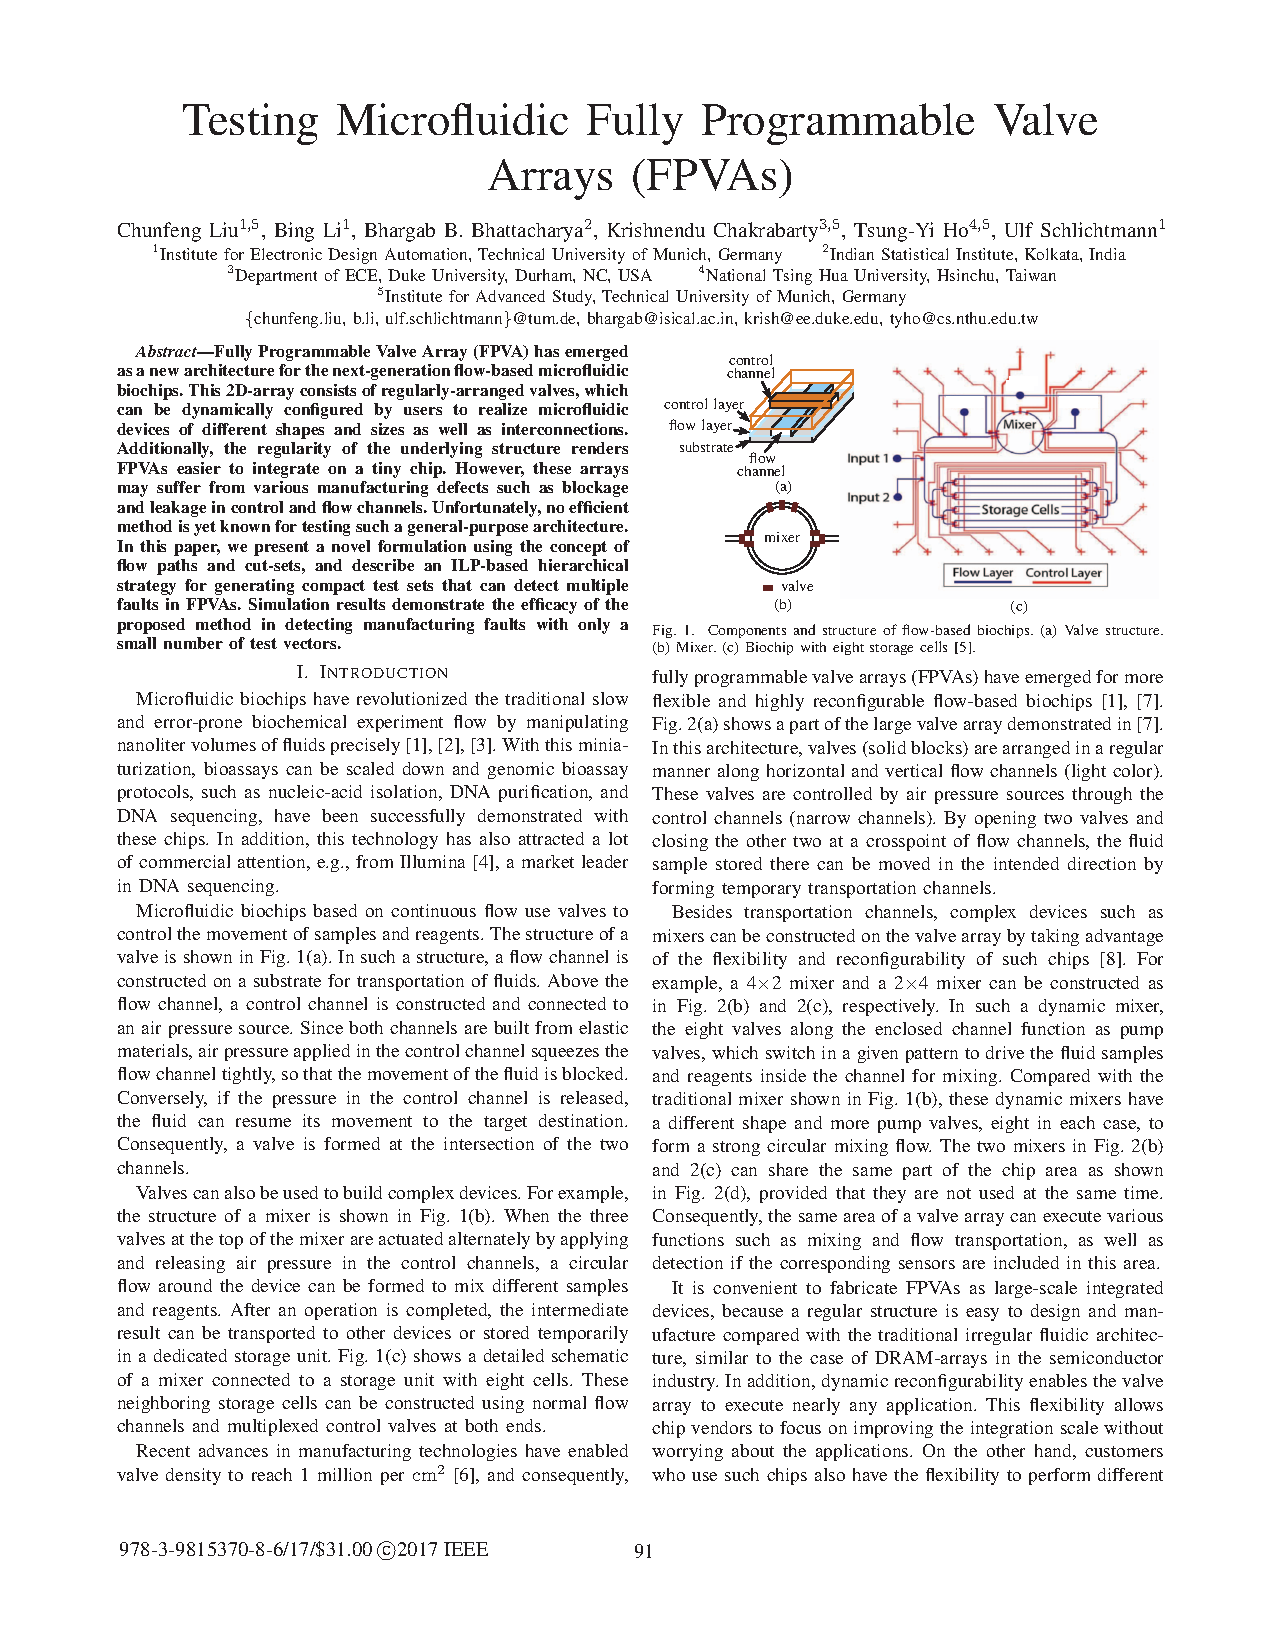
\includepdf[pages=1-last]{07926964.pdf}


\end{document}




